\chapter{Proposed Work}
\section{Introduction}
This chapter outlines the design and methodologies undertaken for the project. The chapter provides detailed explanations beginning with the design phase, including use cases, UML diagrams, and flowcharts.This is followed by a detailed, step-by-step account of each procedure. The chapter concludes with the methods used to evaluate the performance of the Query Assistance.

\section{Project Functionality}
    \subsection{System requirements}
    \begin{itemize}
        \item  Fix SQL query
        \begin{itemize}
            \item Users can input the query along with the error and the database they used.
            \item The system should be able to correct typos in column, table, and schema names.
            \item The system should be able to correct incomplete syntax, including issues like missing or extra commas, parentheses, forgotten keywords, misspelled keywords, incorrect order, and missing keywords.
            \item The system should be able to correct incorrect alias formats and add aliases for improved readability.
            \item The system should be able to correct invalid date formats, mismatched data types, and ambiguous column names.
        \end{itemize}

        \item  Convert SQL query to another database
        \begin{itemize}
            \item Users can input the query and the database syntax they are using, as well as the database syntax they want to convert to.
            \item The system should be able to convert syntax from one database to another within our supported databases.
        \end{itemize}

        \item Optimize SQL query
        \begin{itemize}
            \item Users can input the query and optionally with specific aspects they want to optimize.
            \item The system should be able to optimize the query reducing both time and memory consumption.
        \end{itemize}
        \item Translate natural language to SQL query
        \begin{itemize}
            \item Users can input text to specify the data they want to retrieve.
            \item The system should be able to select the appropriate columns and tables and construct the query without errors, ensuring optimal efficiency.
        \end{itemize}
        \item Supported Database
        \begin{itemize}
            \item Impala
            \item StarRocks
            \item Vertica
            \item Spark
        \end{itemize}
    \end{itemize}
    \subsection{Use Cases Diagram and Narrative}
    \begin{figure}[H]
        \centering
        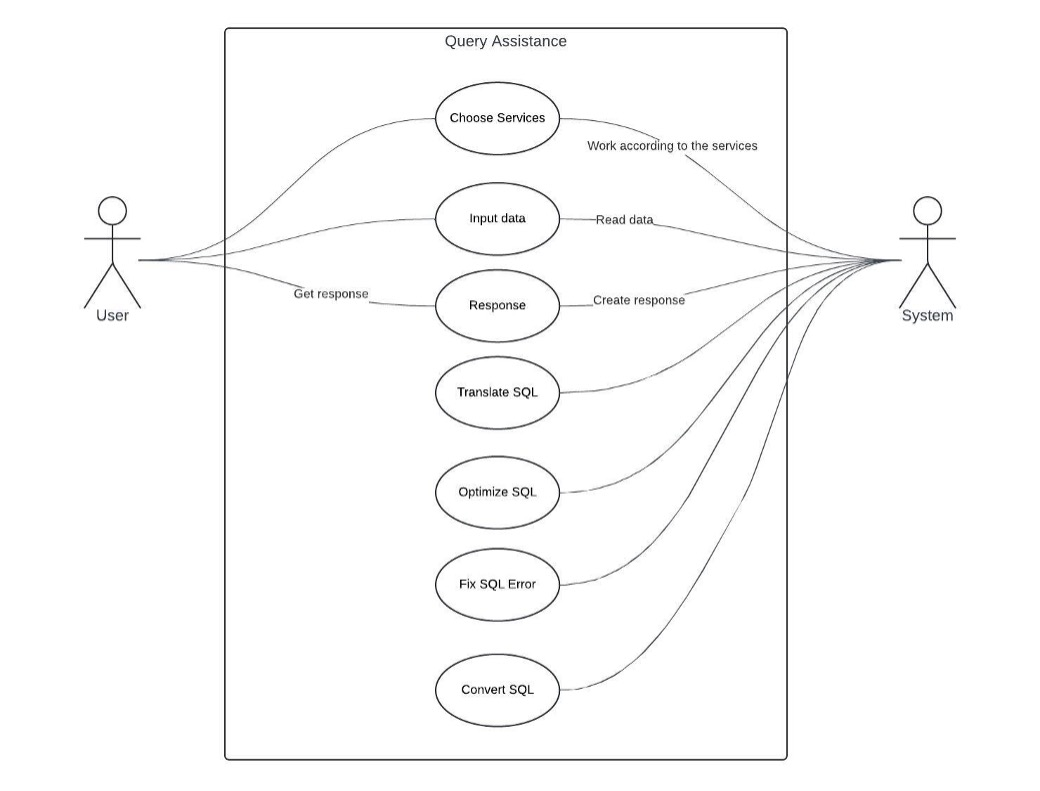
\includegraphics[width=15cm]{chapters/3/figures/usecase_diagram.jpg}
        \caption[Use case diagram of Query Assistance]{Use case diagram of Query Assistance}
        \label{fig:usecase_diagram}
    \end{figure}
    Figure~\ref{fig:usecase_diagram} presents the use case diagram for Query Assistance, visually representing the interactions between the system and its users (actors). It highlights the various functionalities and features available within the Query Assist system, showing how users can engage with it to perform tasks such as generating SQL queries, retrieving data, or integrating with other tools.

    The diagram serves as a high-level overview of the system's capabilities, providing a clear depiction of the relationships between the actors and the system's components. Each use case is further detailed in Tables~\ref{tbl:use-case-fix-sql}-~\ref{tbl:use-case-translate-sql}, where narratives explain the specific functionality, purpose, and flow of each interaction. This comprehensive approach ensures a thorough understanding of how Query Assistance operates and supports user needs. The diagram also emphasizes the flexibility of the system, showcasing its ability to cater to different user roles and scenarios, making it a valuable tool for enhancing productivity and simplifying data-related tasks.

    \begin{table}[H]
        \centering
        \caption{Use case narrative for fix SQL query}
        \label{tbl:use-case-fix-sql}
        \begin{tabular}{|p{4cm}|p{10cm}|}
        \hline
        \textbf{Use Case name} & Fix SQL query \\
        \hline
        \textbf{Actors} & User \\
        \hline
        \textbf{Goal} & Fix SQL Error \\
        \hline
        \textbf{Preconditions} & User has access to the Agoda help platform. \\
        \hline
        \textbf{Main success scenario} &
        \begin{enumerate}
            \item User selects fix query service
            \item User selects query engine
            \item User inputs SQL query and error
            \item System validates the details
            \item System produces the corrected query
        \end{enumerate}
        \\
        \hline
        \textbf{Extension (a)} &
        \begin{enumerate}
            \item[4a.] System validates the details and finds missing required details.
            \item[5a.] System asks the user to fill in the missing required details.
            \item[6a.] Return to step 4
        \end{enumerate}
        \\
        \hline
        \end{tabular}
    \end{table}

    \begin{table}[H]
        \centering
        \caption{Use case narrative for convert SQL query}
        \label{tbl:use-case-convert-sql}
        \begin{tabular}{|p{4cm}|p{10cm}|}
        \hline
        \textbf{Use Case name} & Convert SQL query \\ \hline
        \textbf{Actors} & User \\ \hline
        \textbf{Goal} & Convert SQL to another database syntax \\ \hline
        \textbf{Preconditions} & User has access to the Agoda help platform. \\ \hline
        \textbf{Main success scenario} &
        \begin{enumerate}
            \item User selects convert query service
            \item User selects current query engine
            \item User selects query engine to convert to
            \item System validates the details
            \item System produces the converted query
        \end{enumerate}
        \\ \hline
        \textbf{Extension (a)} &
        \begin{enumerate}
            \item[4a.] System validates the details and finds missing required details.
            \item[5a.] System asks the user to fill in the missing required details.
            \item[6a.] Return to step 4
        \end{enumerate}
        \\ \hline
        \end{tabular}
    \end{table}

    \begin{table}[H]
        \centering
        \caption{Use case narrative for optimize SQL query}
        \label{tbl:use-case-optimize-sql}
        \begin{tabular}{|p{4cm}|p{10cm}|}
        \hline
        \textbf{Use Case name} & Optimize SQL query \\ \hline
        \textbf{Actors} & User \\ \hline
        \textbf{Goal} & Optimize SQL query \\ \hline
        \textbf{Preconditions} & User has access to the Agoda help platform. \\ \hline
        \textbf{Main success scenario} &
        \begin{enumerate}
            \item User selects optimize query service
            \item User selects query engine
            \item User inputs SQL query
            \item System validates the details
            \item System produces the optimized query
        \end{enumerate}
        \\ \hline
        \textbf{Extension (a)} &
        \begin{enumerate}
            \item[4a.] System validates the details and finds missing required details.
            \item[5a.] System asks the user to fill in the missing required details.
            \item[6a.] Return to step 4
        \end{enumerate}
        \\ \hline
        \textbf{Extension (b)} &
        \begin{enumerate}
            \item[3b.] User inputs SQL query and details on optimizing the query
            \item[4b.] Return to step 4
        \end{enumerate}
        \\ \hline
        \end{tabular}
    \end{table}
    \begin{table}[H]
        \centering
        \caption{Use case narrative for translate SQL query}
        \label{tbl:use-case-translate-sql}
        \begin{tabular}{|p{4cm}|p{10cm}|}
        \hline
        \textbf{Use Case name} & Translate SQL query \\ \hline
        \textbf{Actors} & User \\ \hline
        \textbf{Goal} & Translate SQL query \\ \hline
        \textbf{Preconditions} & User has access to the Agoda help platform. \\ \hline
        \textbf{Main success scenario} &
        \begin{enumerate}
            \item User selects translate query service
            \item User selects query engine
            \item User inputs natural language to specify data to retrieve
            \item System validates the details
            \item System produces the SQL query
        \end{enumerate}
        \\ \hline
        \textbf{Extension (a)} &
        \begin{enumerate}
            \item[4a.] System validates the details and finds missing required details.
            \item[5a.] System asks the user to fill in the missing required details.
            \item[6a.] Return to step 4
        \end{enumerate}
        \\ \hline
        \end{tabular}
    \end{table}
\section{System Architecture}
\begin{figure}[H]
    \centering
    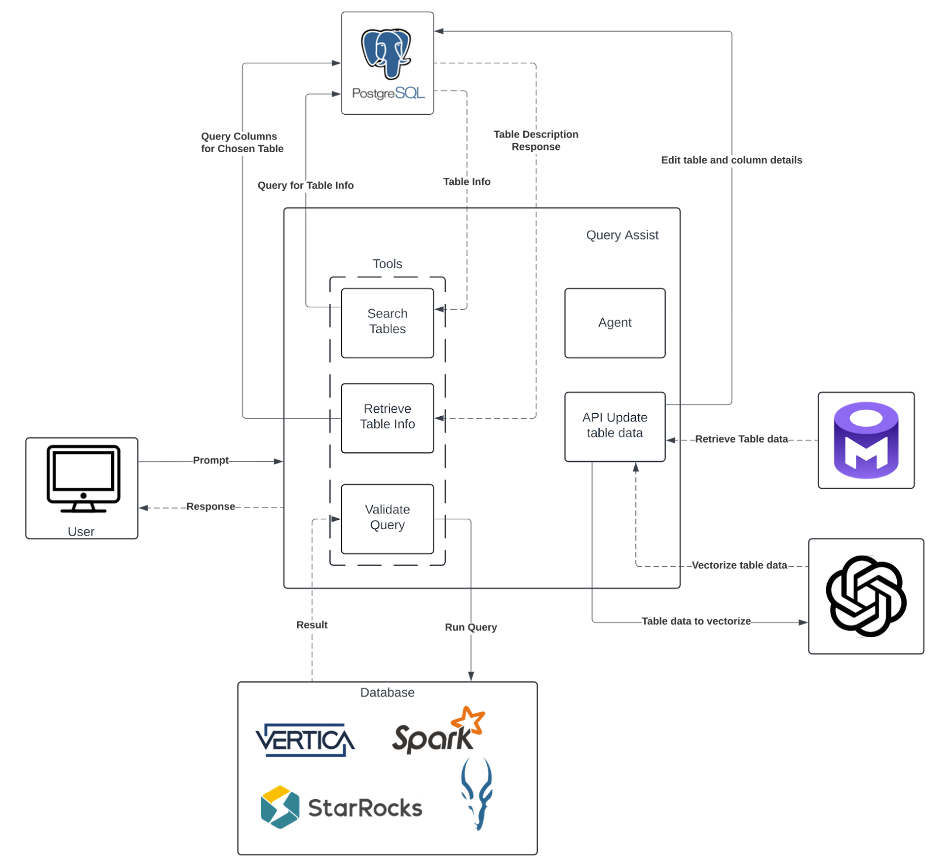
\includegraphics[width=15cm]{chapters/3/figures/architecture.png}
    \caption[Query Assistance Architecture Design]{Query Assistance Architecture Design}
    \label{fig:query_assist_architecture_design}
\end{figure}
Figure~\ref{fig:query_assist_architecture_design} illustrates the relationships between the components in our project. Our system employs a PostgreSQL database to store table and column details, sourcing data from OpenMetaData. When requested, the system retrieves necessary information from the PostgreSQL database, processes it according to user requirements, and generates an SQL statement. Before finalizing and returning the SQL statement, it verifies the statement using the database services provided by the user.

\section{Query Assist Bot}
The Query Assist bot is a Slack bot designed to handle the Slack integration of Query Assist. The bot communicates with Query Assist to send inputs, receive outputs, post results to the Slack channel, collect user feedback, and store all relevant information in the messaging table. In the Agoda Slack community, Opsbot serves as a bot to assist users, meaning that users will always interact with Opsbot when seeking help with queries.

    \subsection{System requirements}
    \begin{itemize}
        \item  The system must make API call to Query Assist whenever it was triggered.
        \item  The system must post the result and feedback form, or error message according to the Query Assist result.
        \item  The system must submit the query assist related data and user feedback to Messaging Table.
        \item  The system must monitor the Slack Channel in order to send feedback to messaging table whenever the submit button of the feedback form is clicked.
    \end{itemize}

    \subsection{System Architecture}
    \begin{figure}[H]
        \centering
        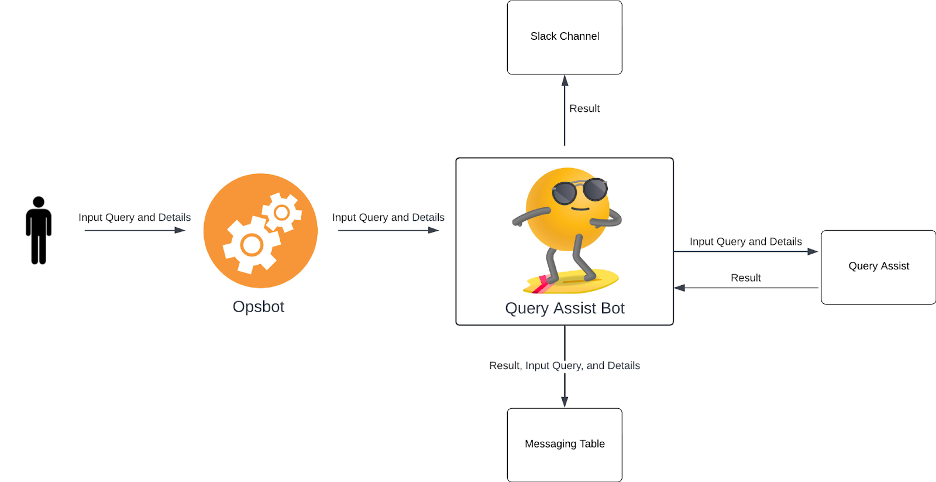
\includegraphics[width=15cm]{chapters/3/figures/bot_architecture.png}
        \caption[Query Assist Bot Architecture Design]{Query Assist Bot Architecture Design}
        \label{fig:bot_architecture_design}
    \end{figure}
    Figure~\ref{fig:bot_architecture_design} illustrates the architectural design of the Query Assist bot and the interactions between its components. The Query Assist bot interacts with four components, namely Opsbot, Slack Channel, Query Assist, and Messaging Table, to achieve its functionality.

    The Query Assist bot is a Slack bot designed to handle the Slack integration of Query Assist. The bot communicates with Query Assist to send inputs, receive outputs, post results to the Slack channel, collect user feedback, and store all relevant information in the messaging table. In the Agoda Slack community, Opsbot serves as a bot to assist users, meaning that users will always interact with Opsbot when seeking help with queries.
    \begin{figure}[H]
        \centering
        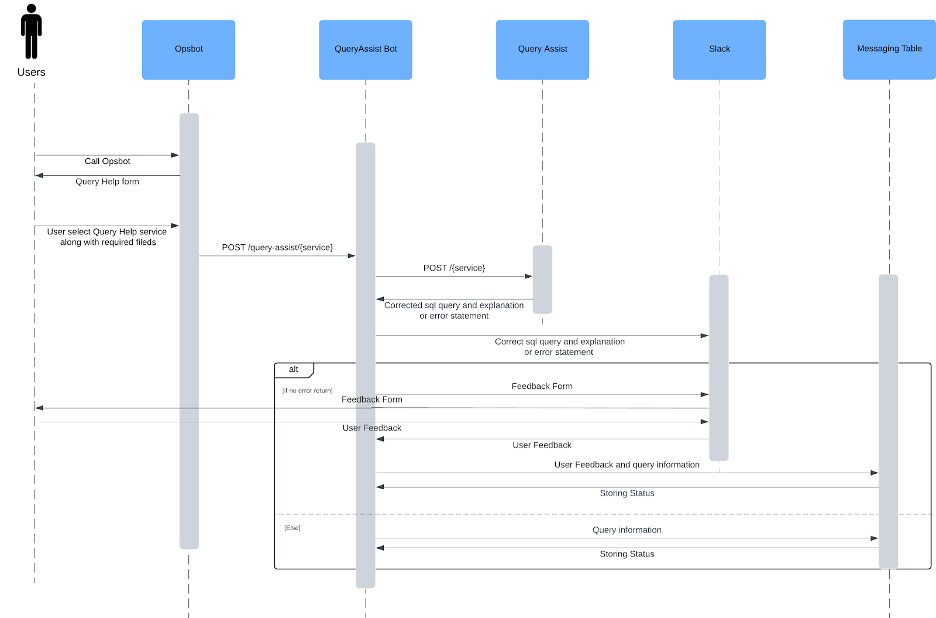
\includegraphics[width=15cm]{chapters/3/figures/sequence_diagram.png}
        \caption[Sequence Diagram of Query Assist Bot]{Sequence Diagram of Query Assist Bot}
        \label{fig:sequence_diagram}
    \end{figure}
    Figure~\ref{fig:sequence_diagram} shows the interaction between the user, Opsbot, Query Assist Bot, Query Assist, Slack and Messaging Table during the process of Query Assist Slack integration.

    Here is the breakdown of the sequence:
    \begin{itemize}
        \item  Step 1: The user initiates the retrieval process by call Opsbot.
        \item  Step 2: Opsbot return the Query Help form for user.
        \item  Step 3: User input all the required field in the form
        \item  Step 4: Opsbot then call Query Assist Bot and send along the required fields
        \item  Step 5: Query Assist bot then call Query Assist and send along the required fields
        \item  Step 6: Query Assist then return the result and explanation or the error statement
        \item  Step 7: Query Assist Bot post the result and explanation or the error statement to Slack channel
        \item  Alternatively, If no error is return:
        \begin{itemize}
            \item Step 7: Query Assist Bot then send feedback form to Slack channel
            \item Step 8: Slack then send the form to user
            \item Step 9: User send the feedback to Slack
            \item Step 10: Slack send feedback to Query Assist Bot
            \item Step 11: Query Assist Bot send user feedback and query information to Messaging Table
            \item Step 12: Messaging return with storing status
        \end{itemize}
        \item  Alternatively, If error is return:
        \begin{itemize}
            \item Step 7: Query Assist Bot send query information to Messaging Table
            \item Step 8: Messaging return with storing status
        \end{itemize}
    \end{itemize}
\section{Update and retrieve metadata}
The update and retrieve metadata component is responsible for storing and retrieving metadata in vector format within PostgreSQL. This metadata is used to verify the integrity of schema, table, and column names. Storing it in vector format allows for efficient similarity comparisons.
\begin{figure}[H]
    \centering
    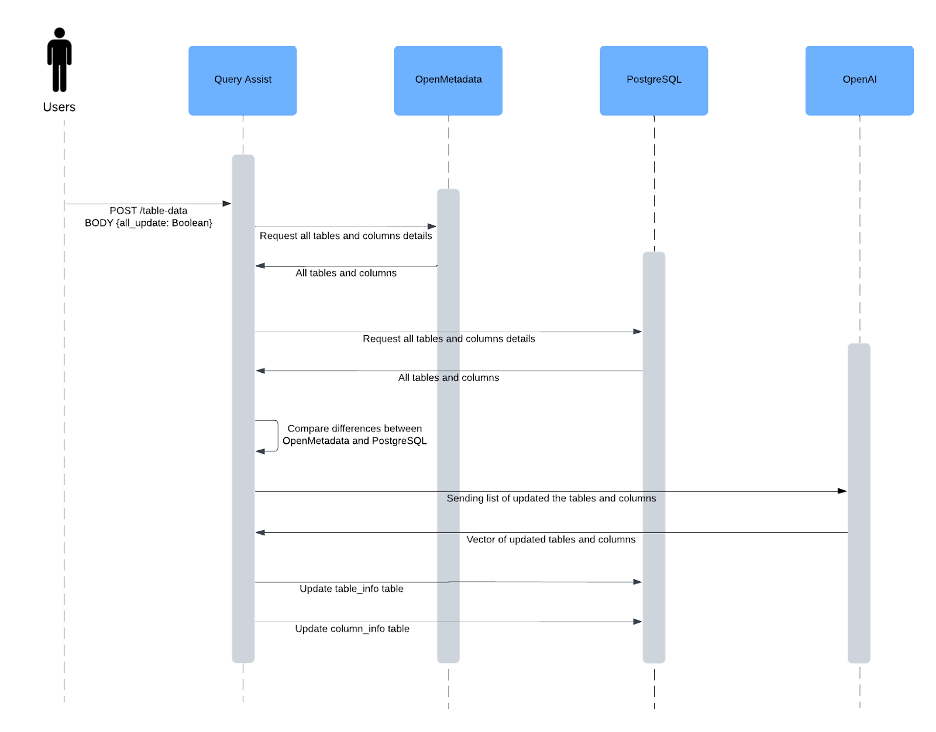
\includegraphics[width=15cm]{chapters/3/figures/retrieve_table.png}
    \caption[Sequence Diagram of Query Assist retrieving metadata]{Sequence Diagram of Query Assist retrieving metadata}
    \label{fig:retrieve_table_sequence_diagram}
\end{figure}
Figure~\ref{fig:retrieve_table_sequence_diagram} shows the interaction between the user, Query Assist, OpenMetadata, PostgreSQL, and OpenAI during the process of retrieving database metadata to use for comparing the integrity of schema, table, and column name.

Here is the breakdown of the sequence:
\begin{itemize}
    \item  Step 1: The user initiates the retrieval process by calling API to Query Assist OpenMetadata
    \item  Step 2: Upon receiving the user's request, the Query Assist sends a request to OpenMetdata, requesting table and column details
    \item  Step 3: OpenMetadata retrieves the data and send the table and column details to the Query Assist back to Query Assist
    \item  Step 4: The Query Assist sends a request to PostgreSQL requesting table and column details that it store
    \item  Step 5: PostgreSQL retrieves the data and send the table and column details to the Query Assist back to Query Assist
    \item  Step 6: Query Assist then compare the differences between Openmeta and PostgreSQL to look for the data that is not yet available in PostgreSQL but available in the OpenMetada
    \item  Step 7: Query Assist then sending the list of updated the table and column to OpenAI
    \item  Step 8: OpenAI then embedded and send the vector of updated the table and column back to Query Assist
    \item  Step 9:  Query Assist update the table\_info in the PostgreSQL according to the updated list
    \item  Step 10: Query Assist update the column\_info in the PostgreSQL according to the updated list
\end{itemize}

\section{Tools}
    \subsection{Search Table}
    \begin{figure}[H]
        \centering
        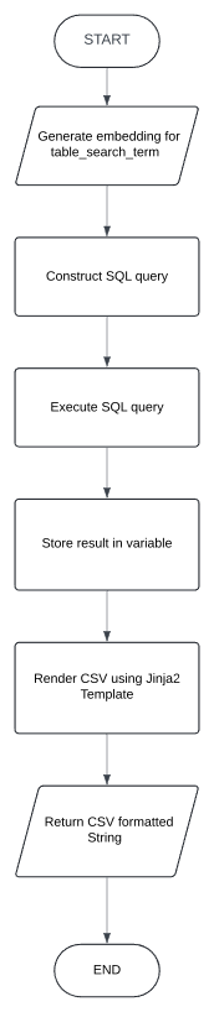
\includegraphics[width=3cm]{chapters/3/figures/search_table.png}
        \caption[Search Table’s flowchart]{Search Table’s flowchart}
        \label{fig:search_table}
    \end{figure}
    Figure~\ref{fig:search_table} illustrates the Search Table Tool workflow. It is a tool designed to efficiently retrieve tables from the database. It provides information such as the schema, table name, description, impression, and distance. The agent interacts with this tool by using the desired table name as input. This name is embedded into a vector that facilitates the retrieval process by identifying tables in the database with the closest resemblance to the provided name. This functionality enables agents to get table information to perform constructing the query.

    Here is the breakdown of the flow:
    \begin{itemize}
        \item  Embedding table\_search\_term for familiarity search
        \item  Construct query with embedded data for similarity search
        \item  Execute constructed query
        \item  Store information in data structure
        \item  Render data in CSV using Jinja2 Template
        \item  Return result in CSV formatted string
    \end{itemize}

    \subsection{Retrieve Table Information}
    \label{sec:retrieve_table_info}
    \begin{figure}[H]
        \centering
        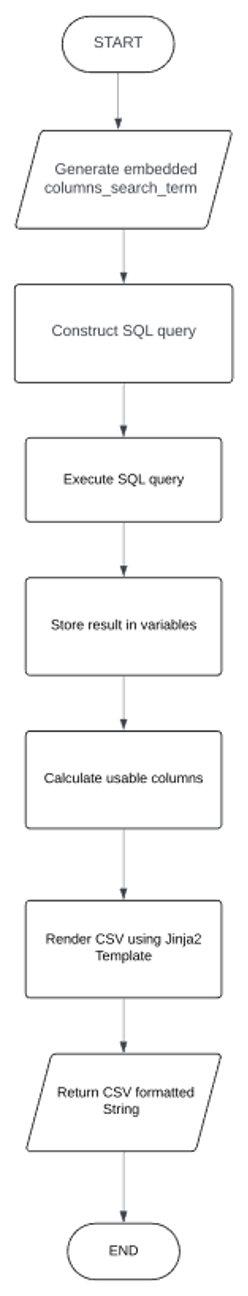
\includegraphics[width=3cm]{chapters/3/figures/retrieve_table_info.png}
        \caption[Retrieve Table Information's flowchart]{Retrieve Table Information's flowchart}
        \label{fig:retrieve_table_info}
    \end{figure}
    Figure~\ref{fig:retrieve_table_info} illustrates the  Retrieve Table tool workflow which is one of the significant tools used within the Query Assist. Retrieve Table Information focused on retrieving column data of specific tables. This function provided table information and details of columns in the table included column name, data type, and description of column.

    Here is the breakdown of the flow:
    \begin{itemize}
        \item  Embedding column\_search\_term for familiarity search
        \item  Construct query with schema and table name
        \item  Execute constructed query
        \item  Store information in data structure
        \item  Find similarity between each column and embedded vector
        \item  Render data in CSV using Jinja2 Template
        \item  Return result in CSV formatted string
    \end{itemize}

    \subsection{Validate Query}
    \begin{figure}[H]
        \centering
        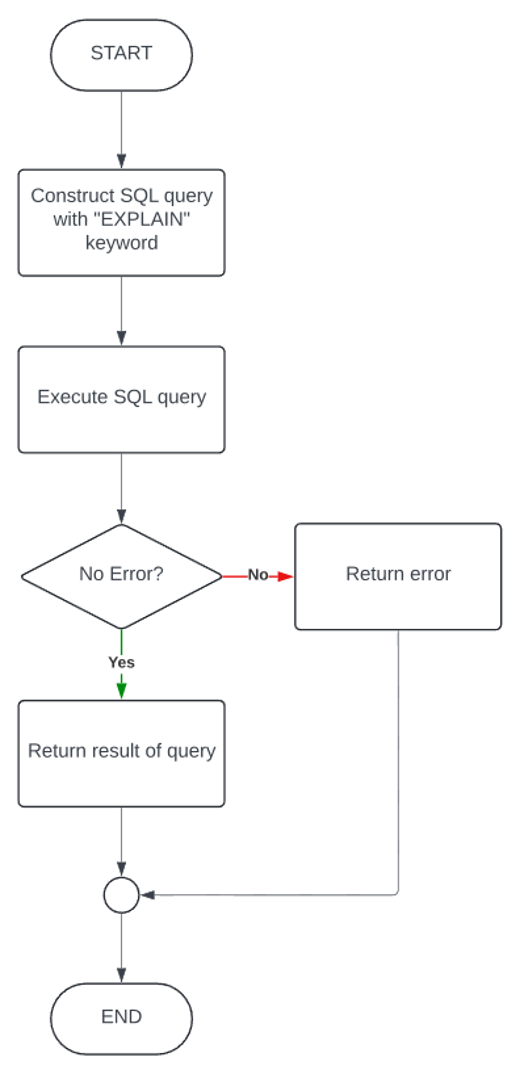
\includegraphics[width=6cm]{chapters/3/figures/validate.png}
        \caption[Validate Query’s flowchart]{Validate Query’s flowchart}
        \label{fig:validate}
    \end{figure}
    Figure~\ref{fig:validate} illustrates the workflow of the Validate Query tool. Validate query is the tool to check whether the query is executable or not. The tool will use the query given by the agent to execute which added the ‘EXPLAIN’ keyword into the query.

    Here is the breakdown of the flow:
    \begin{itemize}
        \item  Construct a query with an 'EXPLAIN' keyword.
        \item  Execute the query
        \item  Return result of the query if query has no error
        \item  Return error of the query if query has error
    \end{itemize}

    \subsection{Column Validation}
    \label{sec:column_validation}
    \begin{figure}[H]
        \centering
        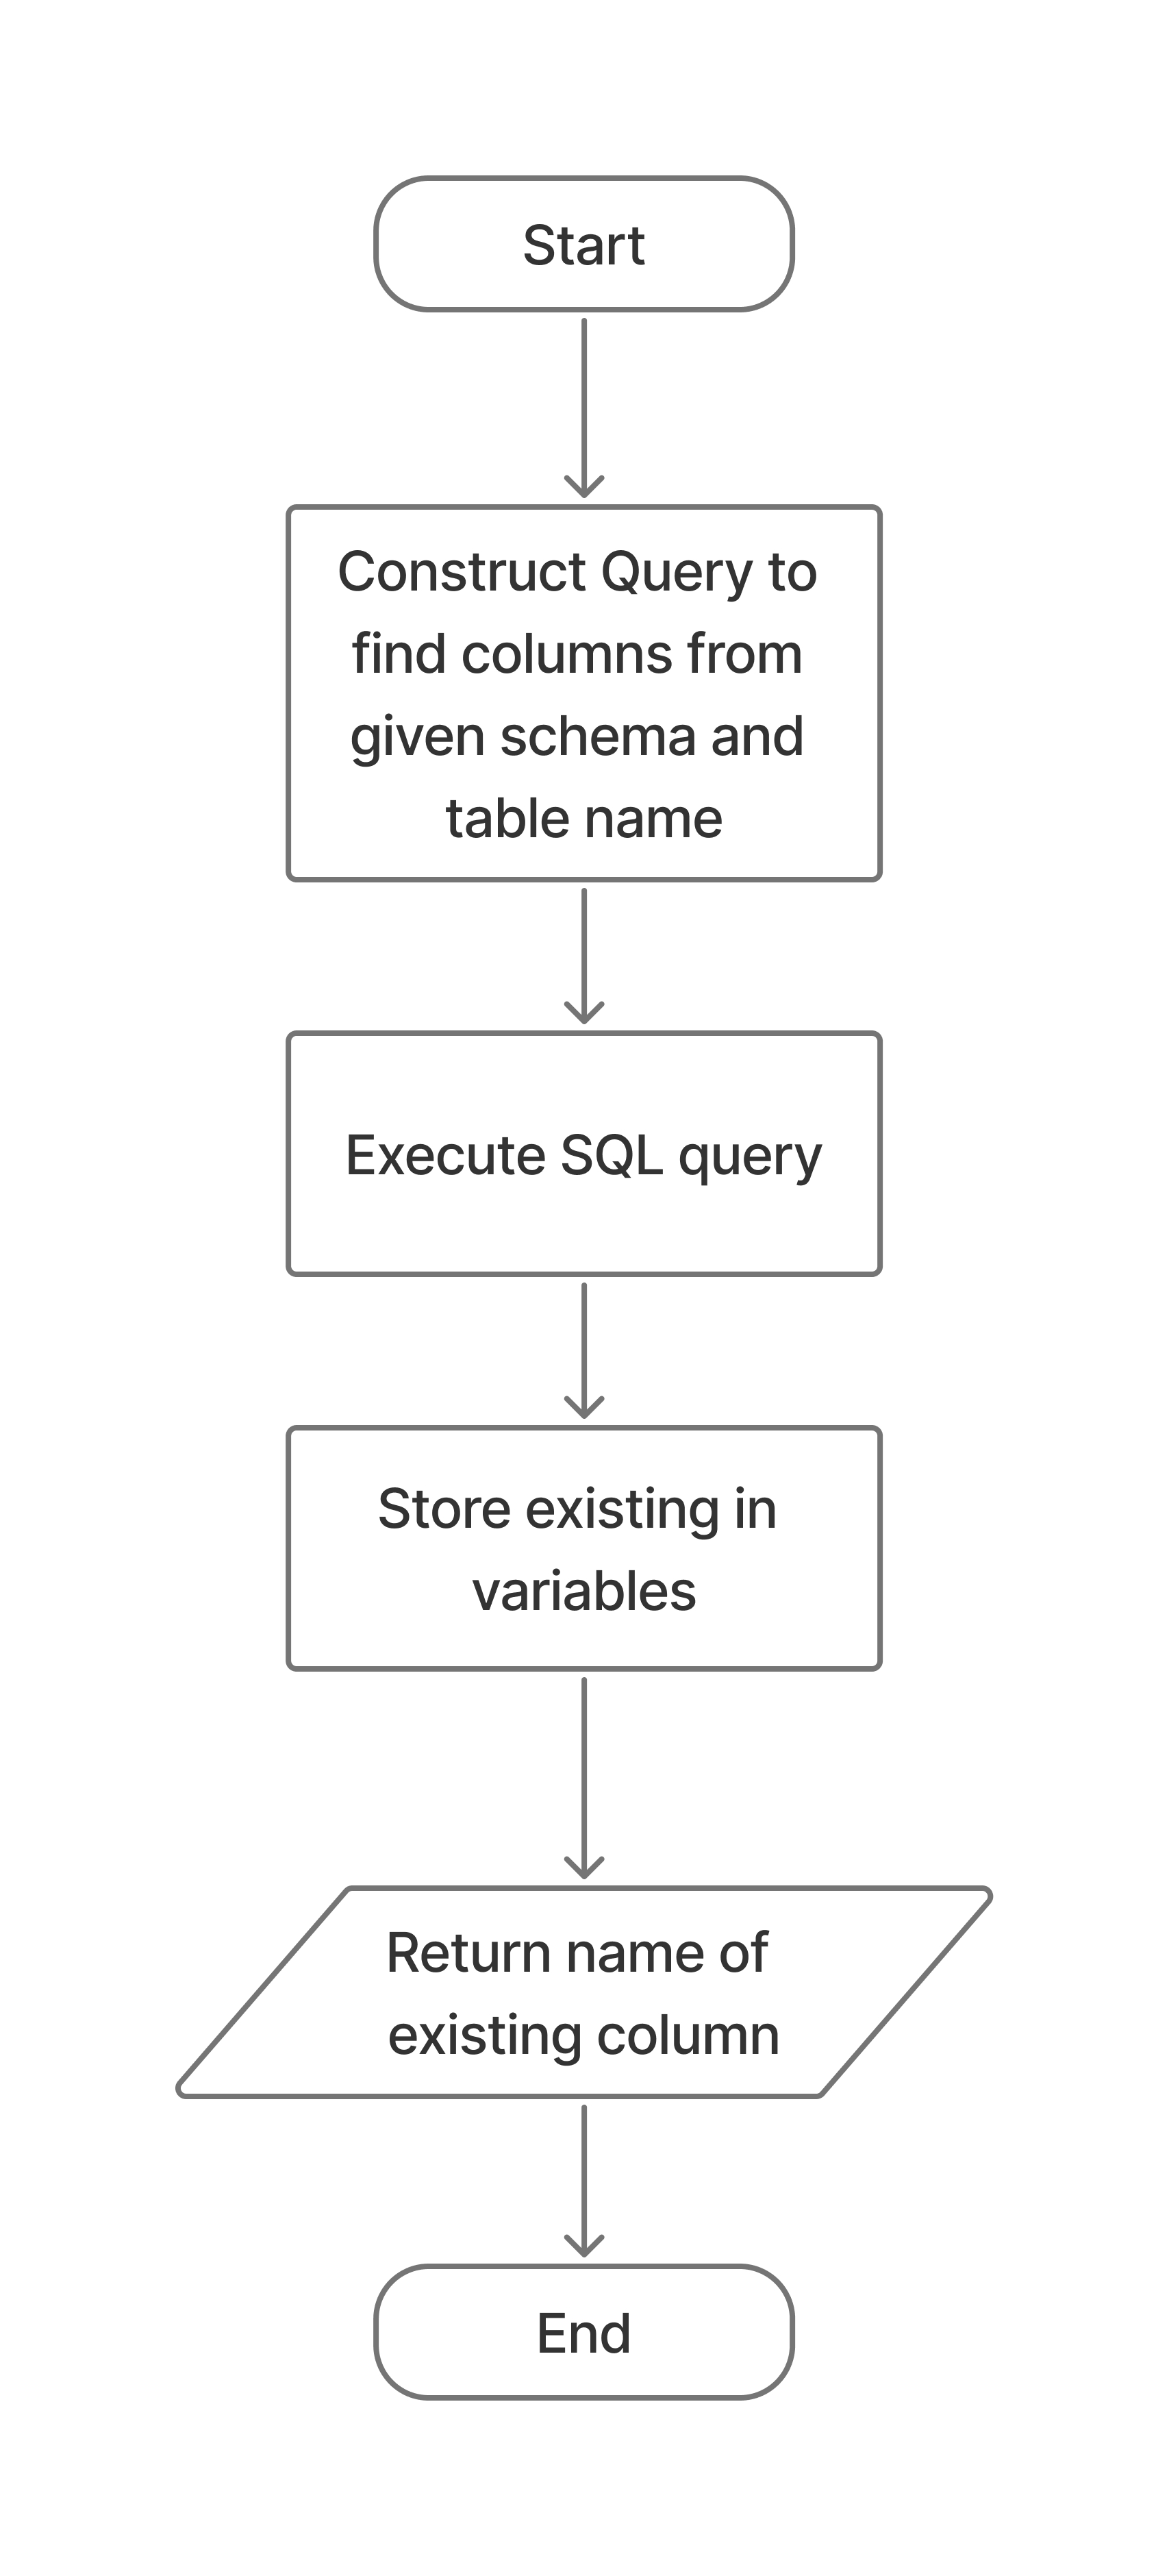
\includegraphics[width=5cm]{chapters/3/figures/column_validate.jpg}
        \caption[Column Validation tool’s flowchart]{Column Validation tool’s flowchart}
        \label{fig:column_validate}
    \end{figure}
    Figure~\ref{fig:column_validate} illustrates the workflow of the Column Validation tool. This tool is used to verify whether the columns provided by the agent actually exist. The tool outputs all columns that are present in the table.
    Here is the breakdown of the flow:
    \begin{itemize}
        \item  Construct a query to find all columns.
        \item  Execute the query
        \item  Store existing column in variable
        \item  Return all the column name that exist
    \end{itemize}

    \subsection{Retrive Partition Column}
    \begin{figure}[H]
        \centering
        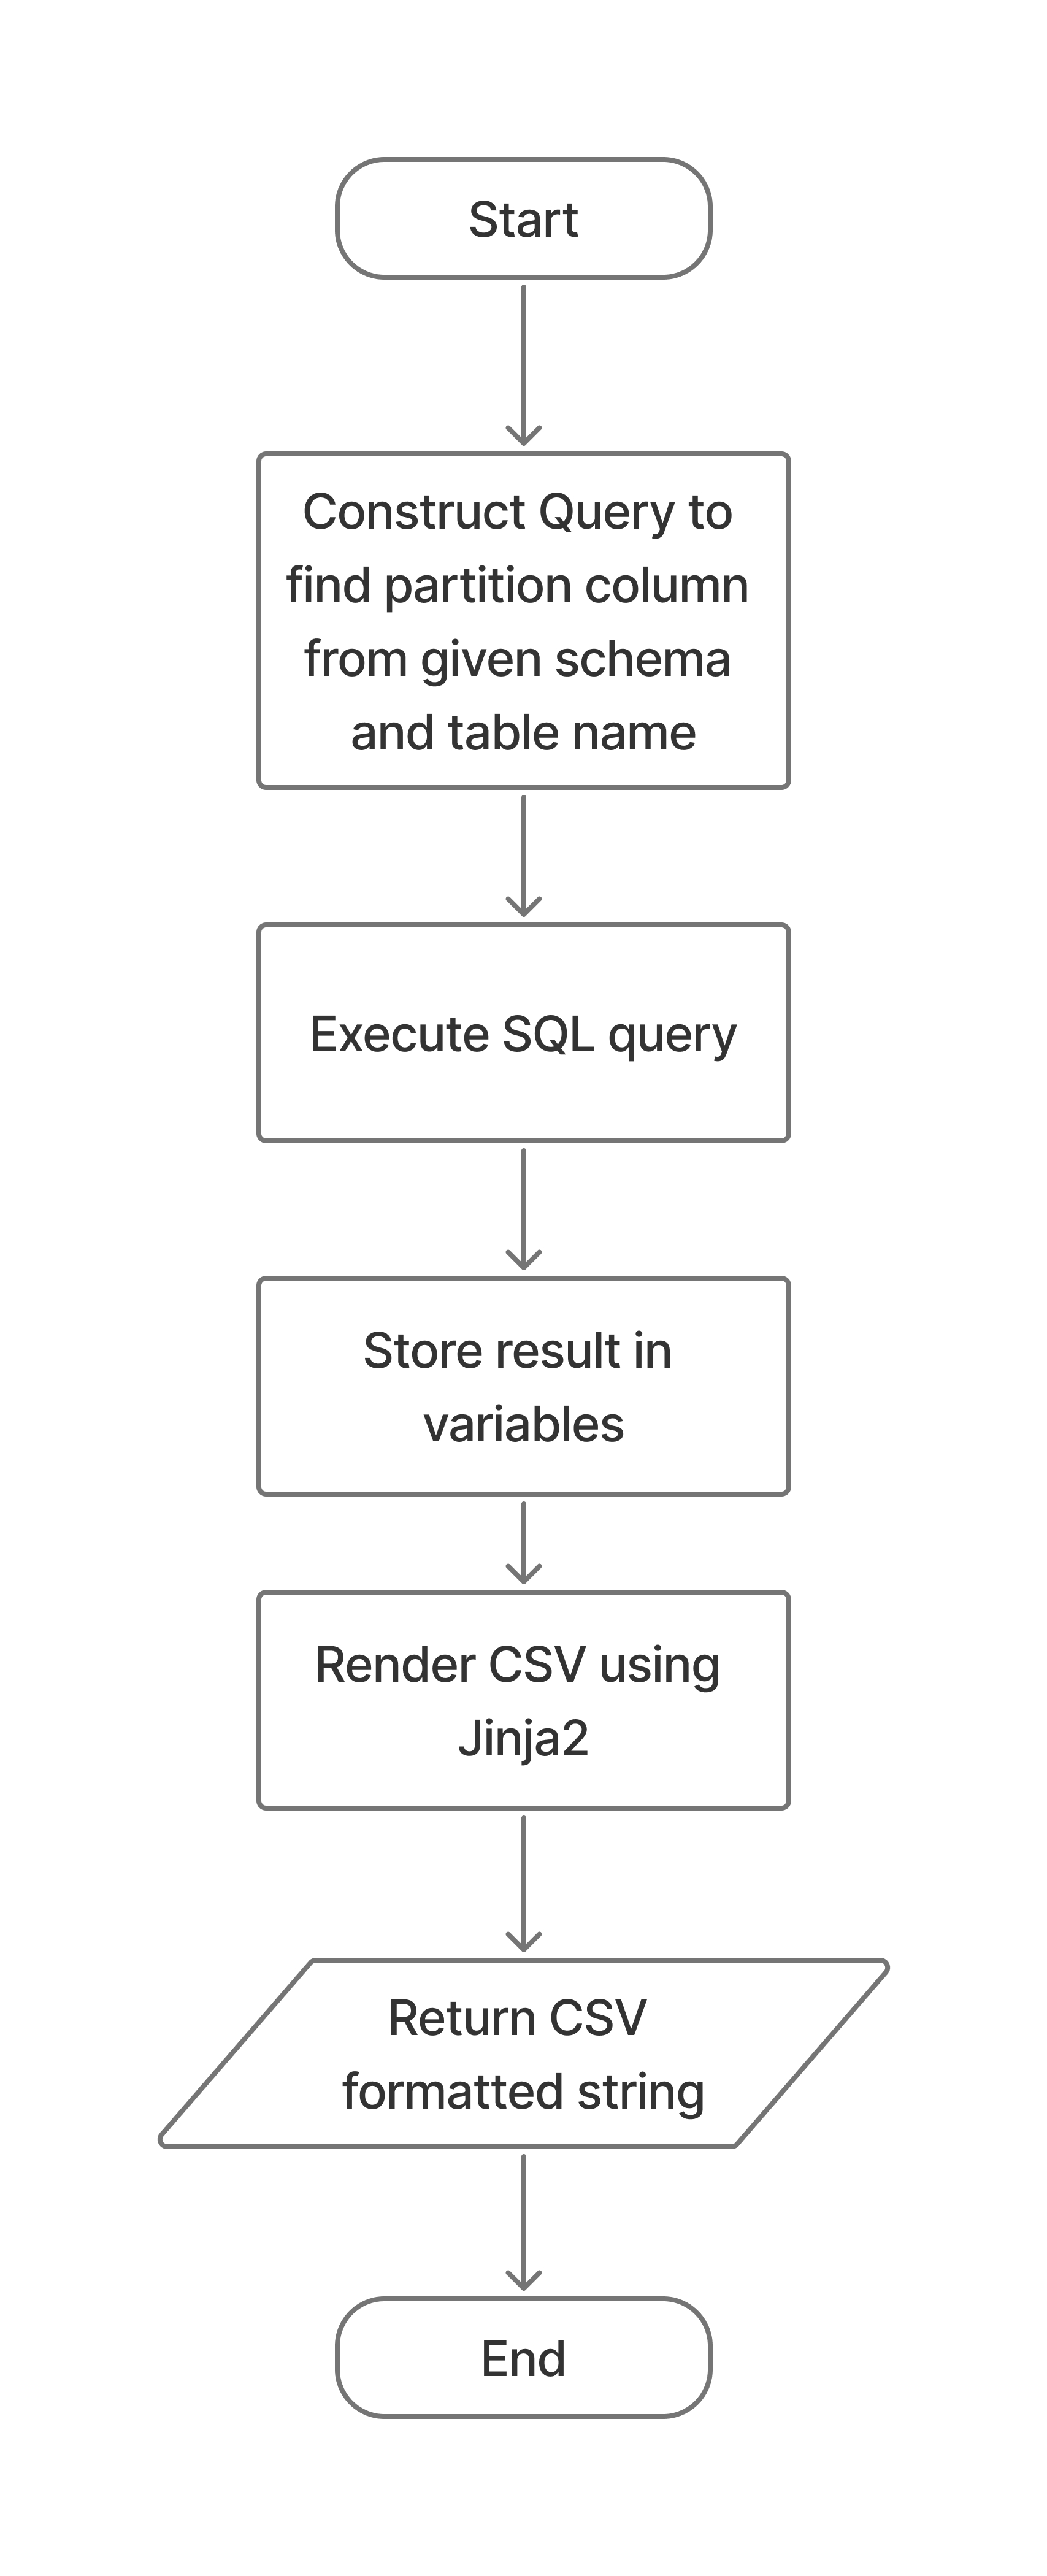
\includegraphics[width=5cm]{chapters/3/figures/partition_columns.jpg}
        \caption[Retrieve Partition Columns’s flowchart]{Retrieve Partition Columns’s flowchart}
        \label{fig:partition_column}
    \end{figure}
    Figure~\ref{fig:partition_column} illustrates the workflow of the Retrieve Partition Columns tool. Retrieve Partition Columns is the tool to retrieve the partition columns of the given schema and table name. The tool is used to the the basic optimization of the query so that it does not consume too much resources.
    Here is the breakdown of the flow:
    \begin{itemize}
        \item  Construct a query to find partition columns.
        \item  Execute the query
        \item  Store information in data structure
        \item  Render data in CSV using Jinja2 Template
        \item  Return result in CSV formatted string
    \end{itemize}

    \subsection{Find Reserved Keyword}
    \begin{figure}[H]
        \centering
        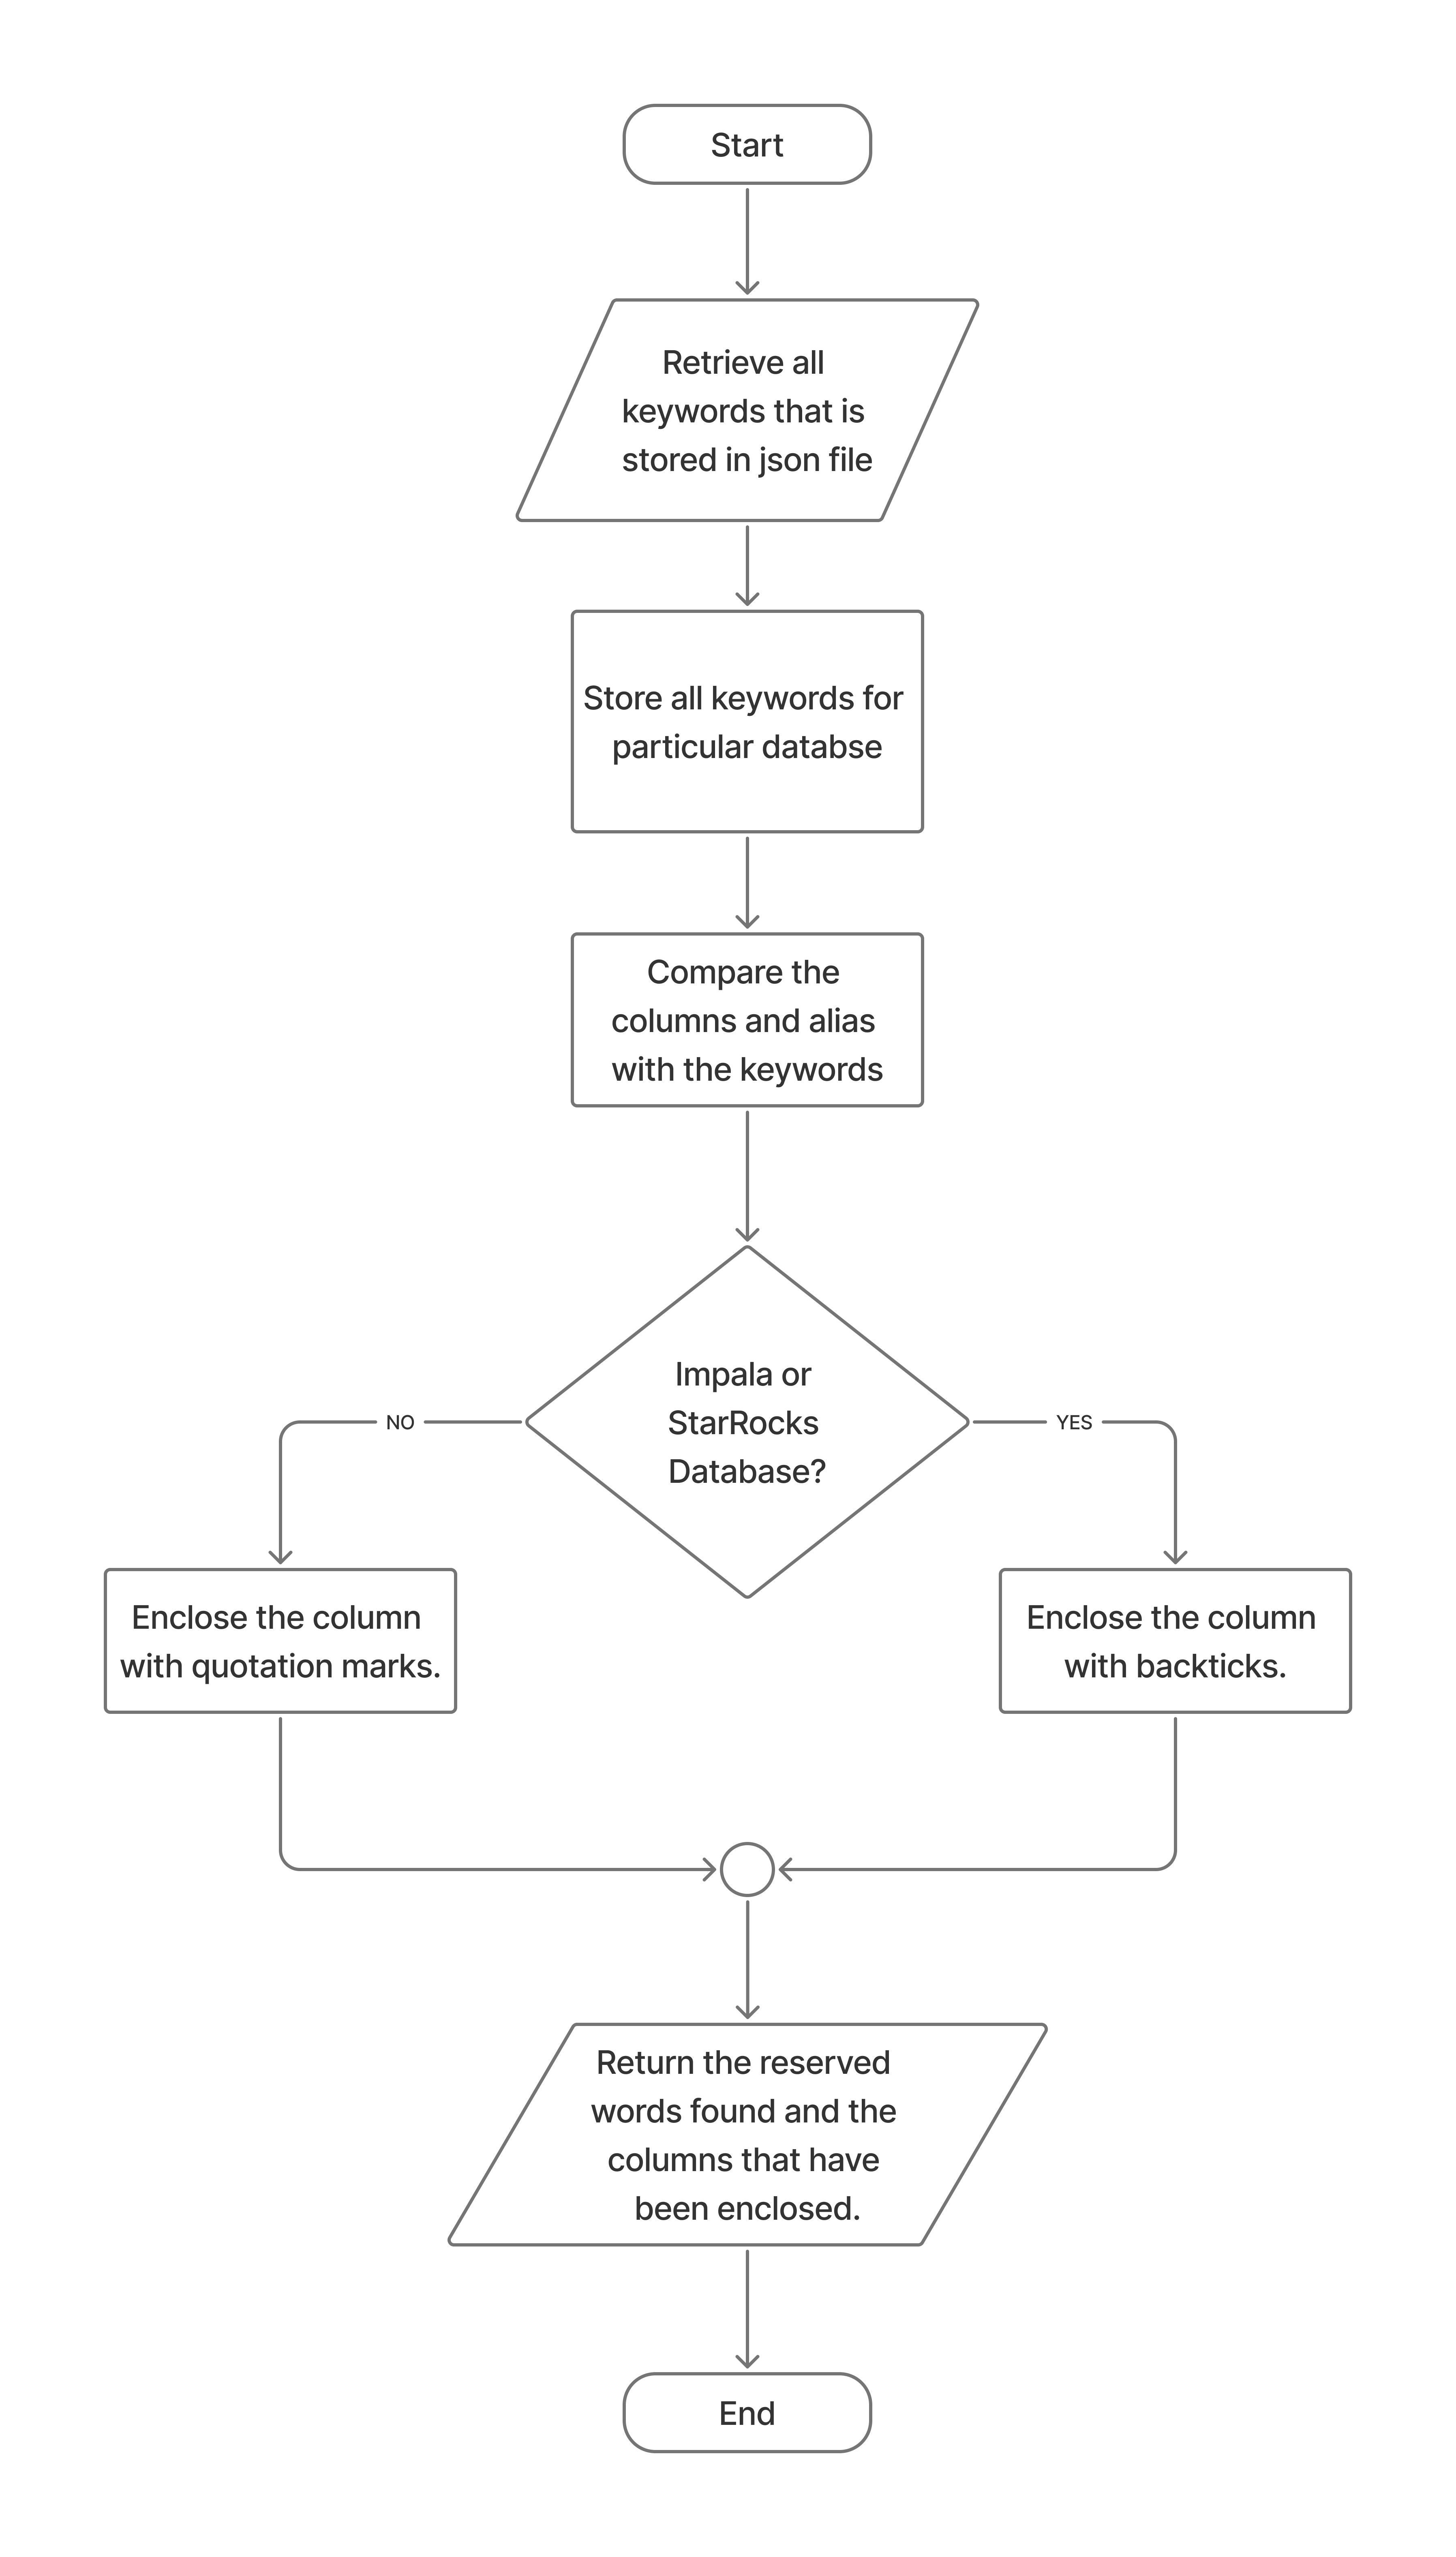
\includegraphics[width=7cm]{chapters/3/figures/reserved_words.jpg}
        \caption[Find Reserved Keyword’s flowchart]{Find Reserved Keyword’s flowchart}
        \label{fig:reserved_words}
    \end{figure}
    Figure~\ref{fig:reserved_words} illustrates the workflow of the Find Reserved Keyword tool. Find Reserved Keyword is the tool to find the reserved words that is used as aliases or column names within the query. These reserved words can cause the error in the query and needed to be handle properly.
    Here is the breakdown of the flow:
    \begin{itemize}
        \item  Retrieve the list of reserved words from the json file
        \item  Store the list of reserved words in a data structure of the given database
        \item  Compare the column names and aliases with the reserved words
        \item  Enclose the column names and aliases in double quotes if you are using StarRocks or Impala, or in backticks if you are using Vertica, whenever they are reserved words.
        \item  Return all the reserved words that are used in the query and the column names and aliases that are enclosed with double quotes or backticks
    \end{itemize}

    \subsection{Handle array, struct, and map column data types}
    \begin{figure}[H]
        \centering
        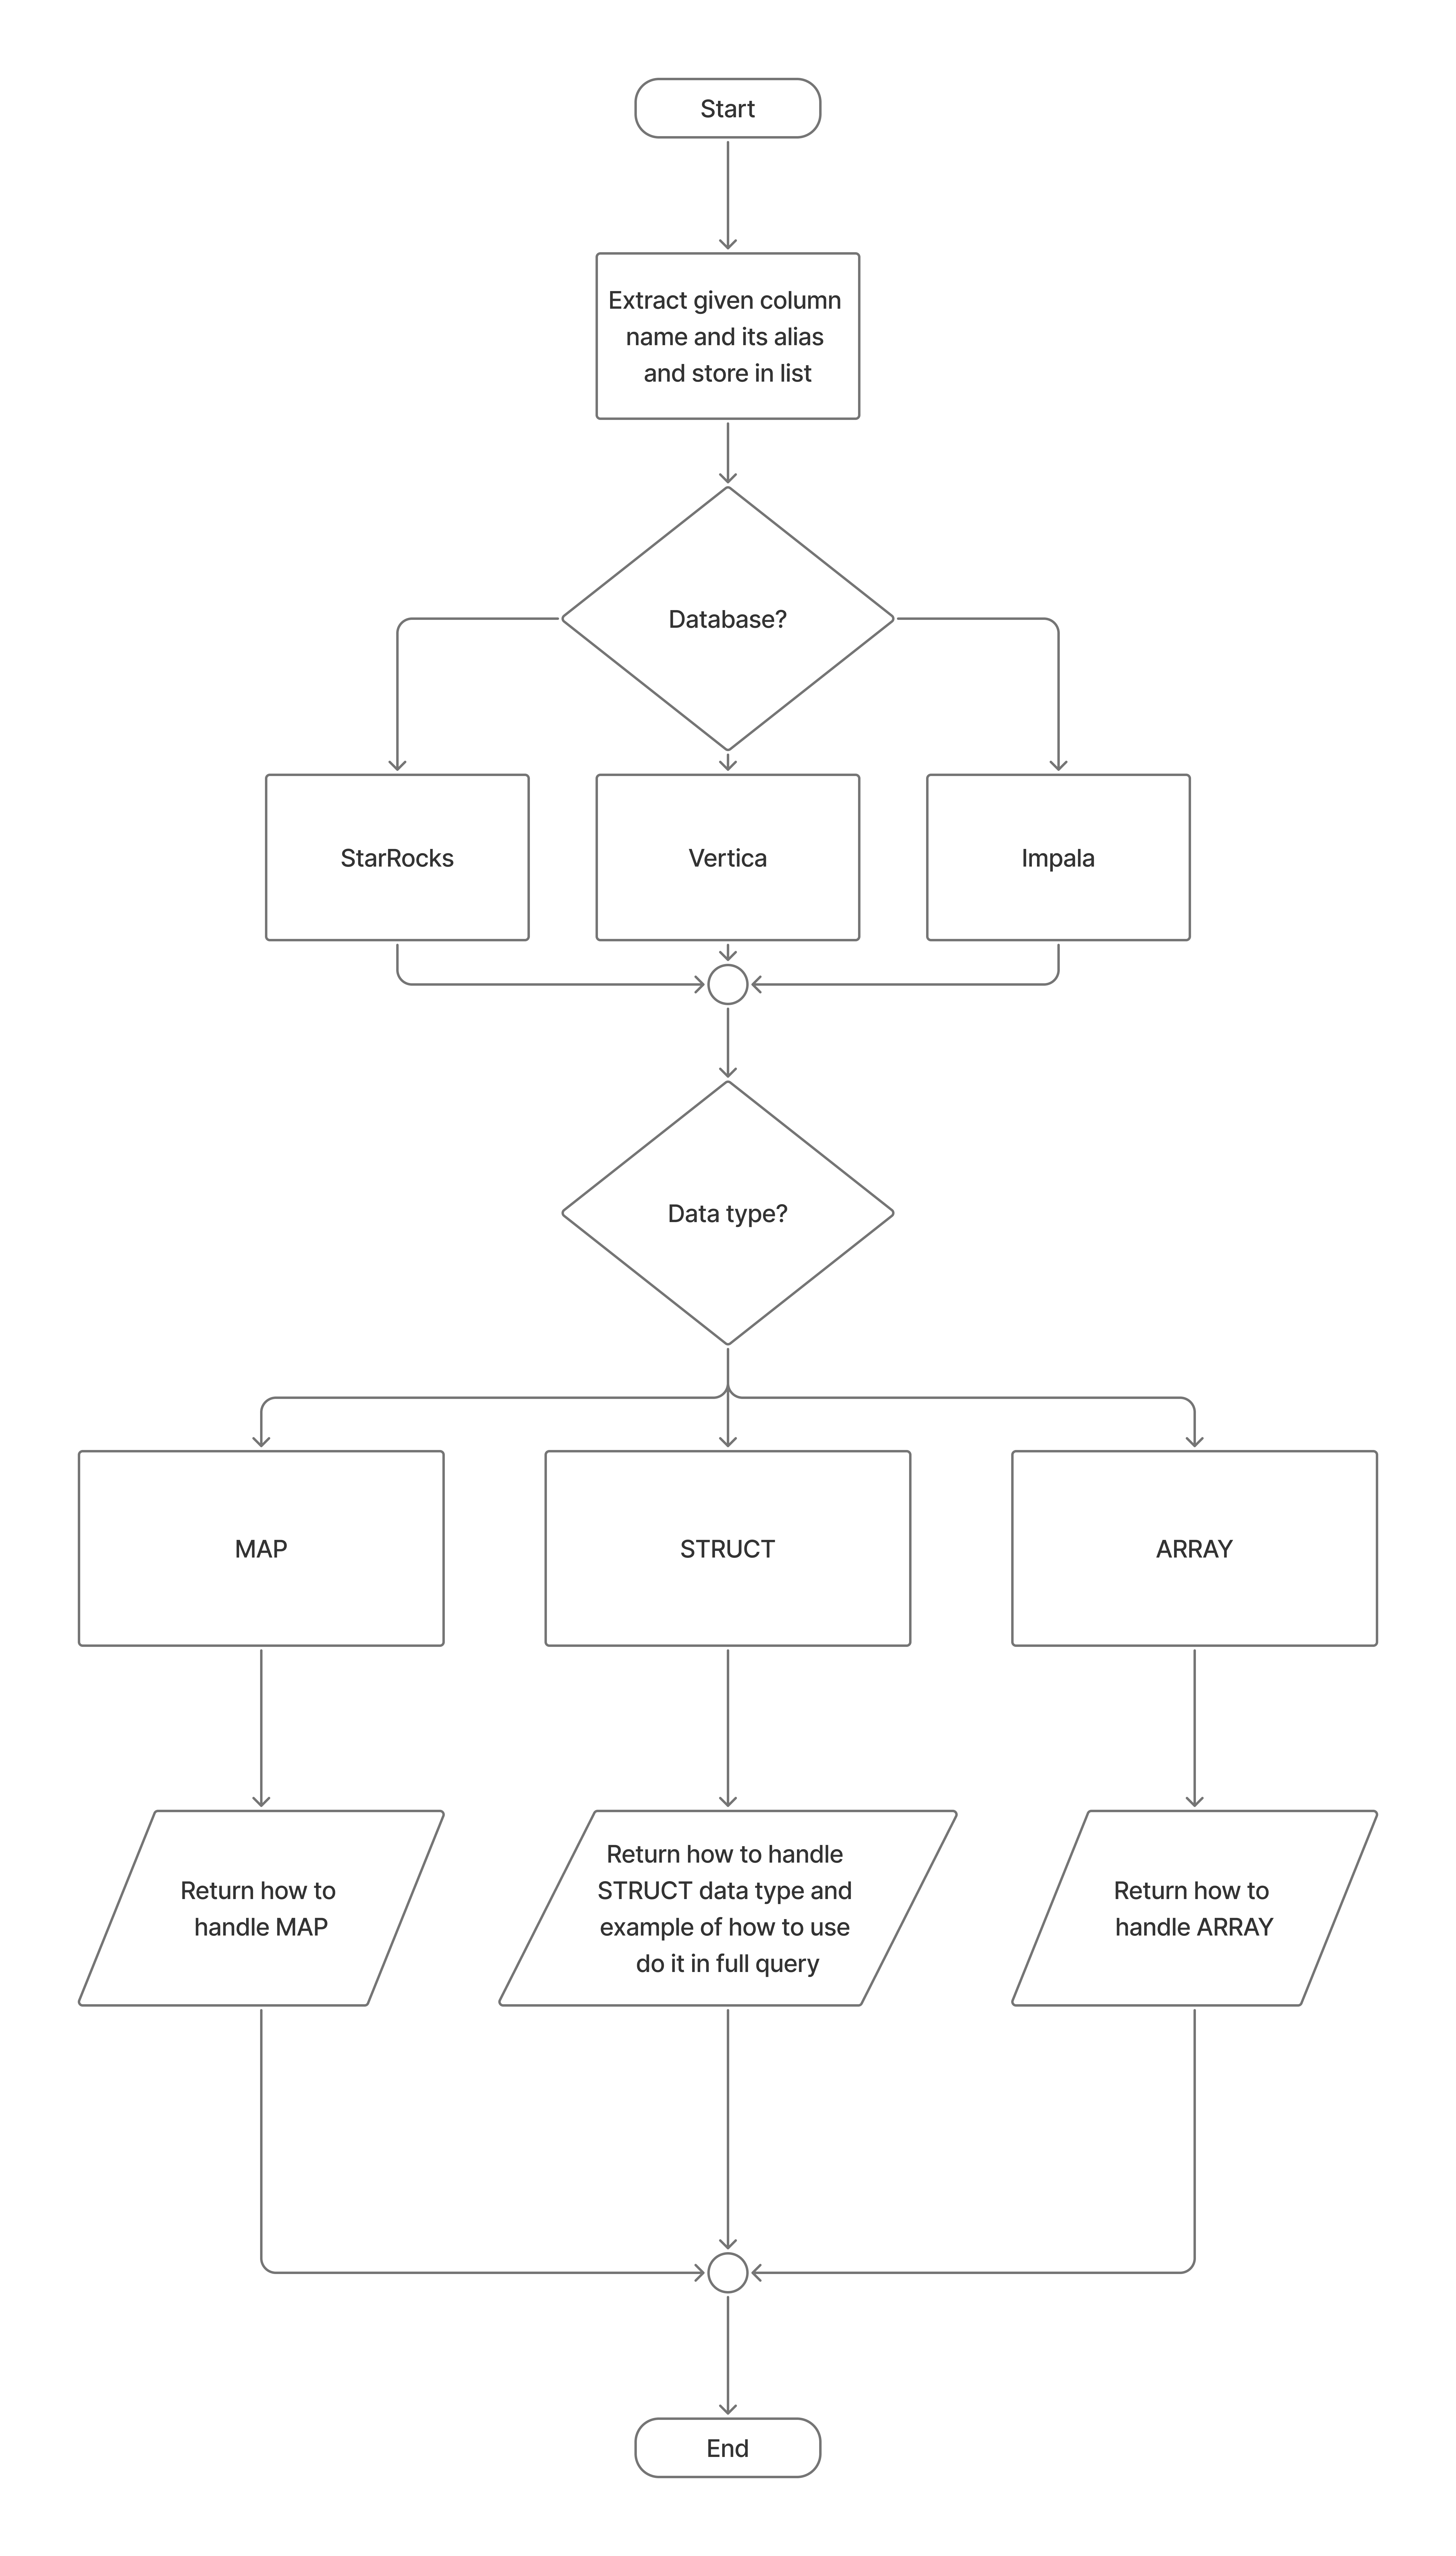
\includegraphics[width=7cm]{chapters/3/figures/array_struct.jpg}
        \caption[Handle array, struct, and map column data types tool’s flowchart]{Handle array, struct, and map column data types tool’s flowchart}
        \label{fig:array_struct}
    \end{figure}
    Figure~\ref{fig:array_struct} illustrates the workflow of the Handle array, struct, and map column data types tool. Handle array, struct, and map column data types is the tool to assists the agent in properly handling these complex data types, as they often require special attention and detailed steps to retrieve and process them correctly.
    Here is the breakdown of the flow:
    \begin{itemize}
        \item  The tool extracts the column name and its alias from the input and stores them in a list for further processing.
        \item  The tool checks which database is being used. The options are: StarRocks, Vertica, and Impala
        \item  Regardless of which database is selected, the process continues to checks the data type of the column. The options are: MAP, STRUCT, and ARRAY
        \item  Depending on the data type, the tool takes a different action:
        \begin{itemize}
            \item MAP: The tool returns instructions on how to handle the MAP data type.
            \item STRUCT: The tool returns instructions on how to handle the STRUCT data type, including an example of how to use it in a full query.
            \item ARRAY:The tool returns instructions on how to handle the ARRAY data type.
        \end{itemize}
    \end{itemize}

    \subsection{Retrieve table in workspace}
    \label{sec:table_in_workspace}
    \begin{figure}[H]
        \centering
        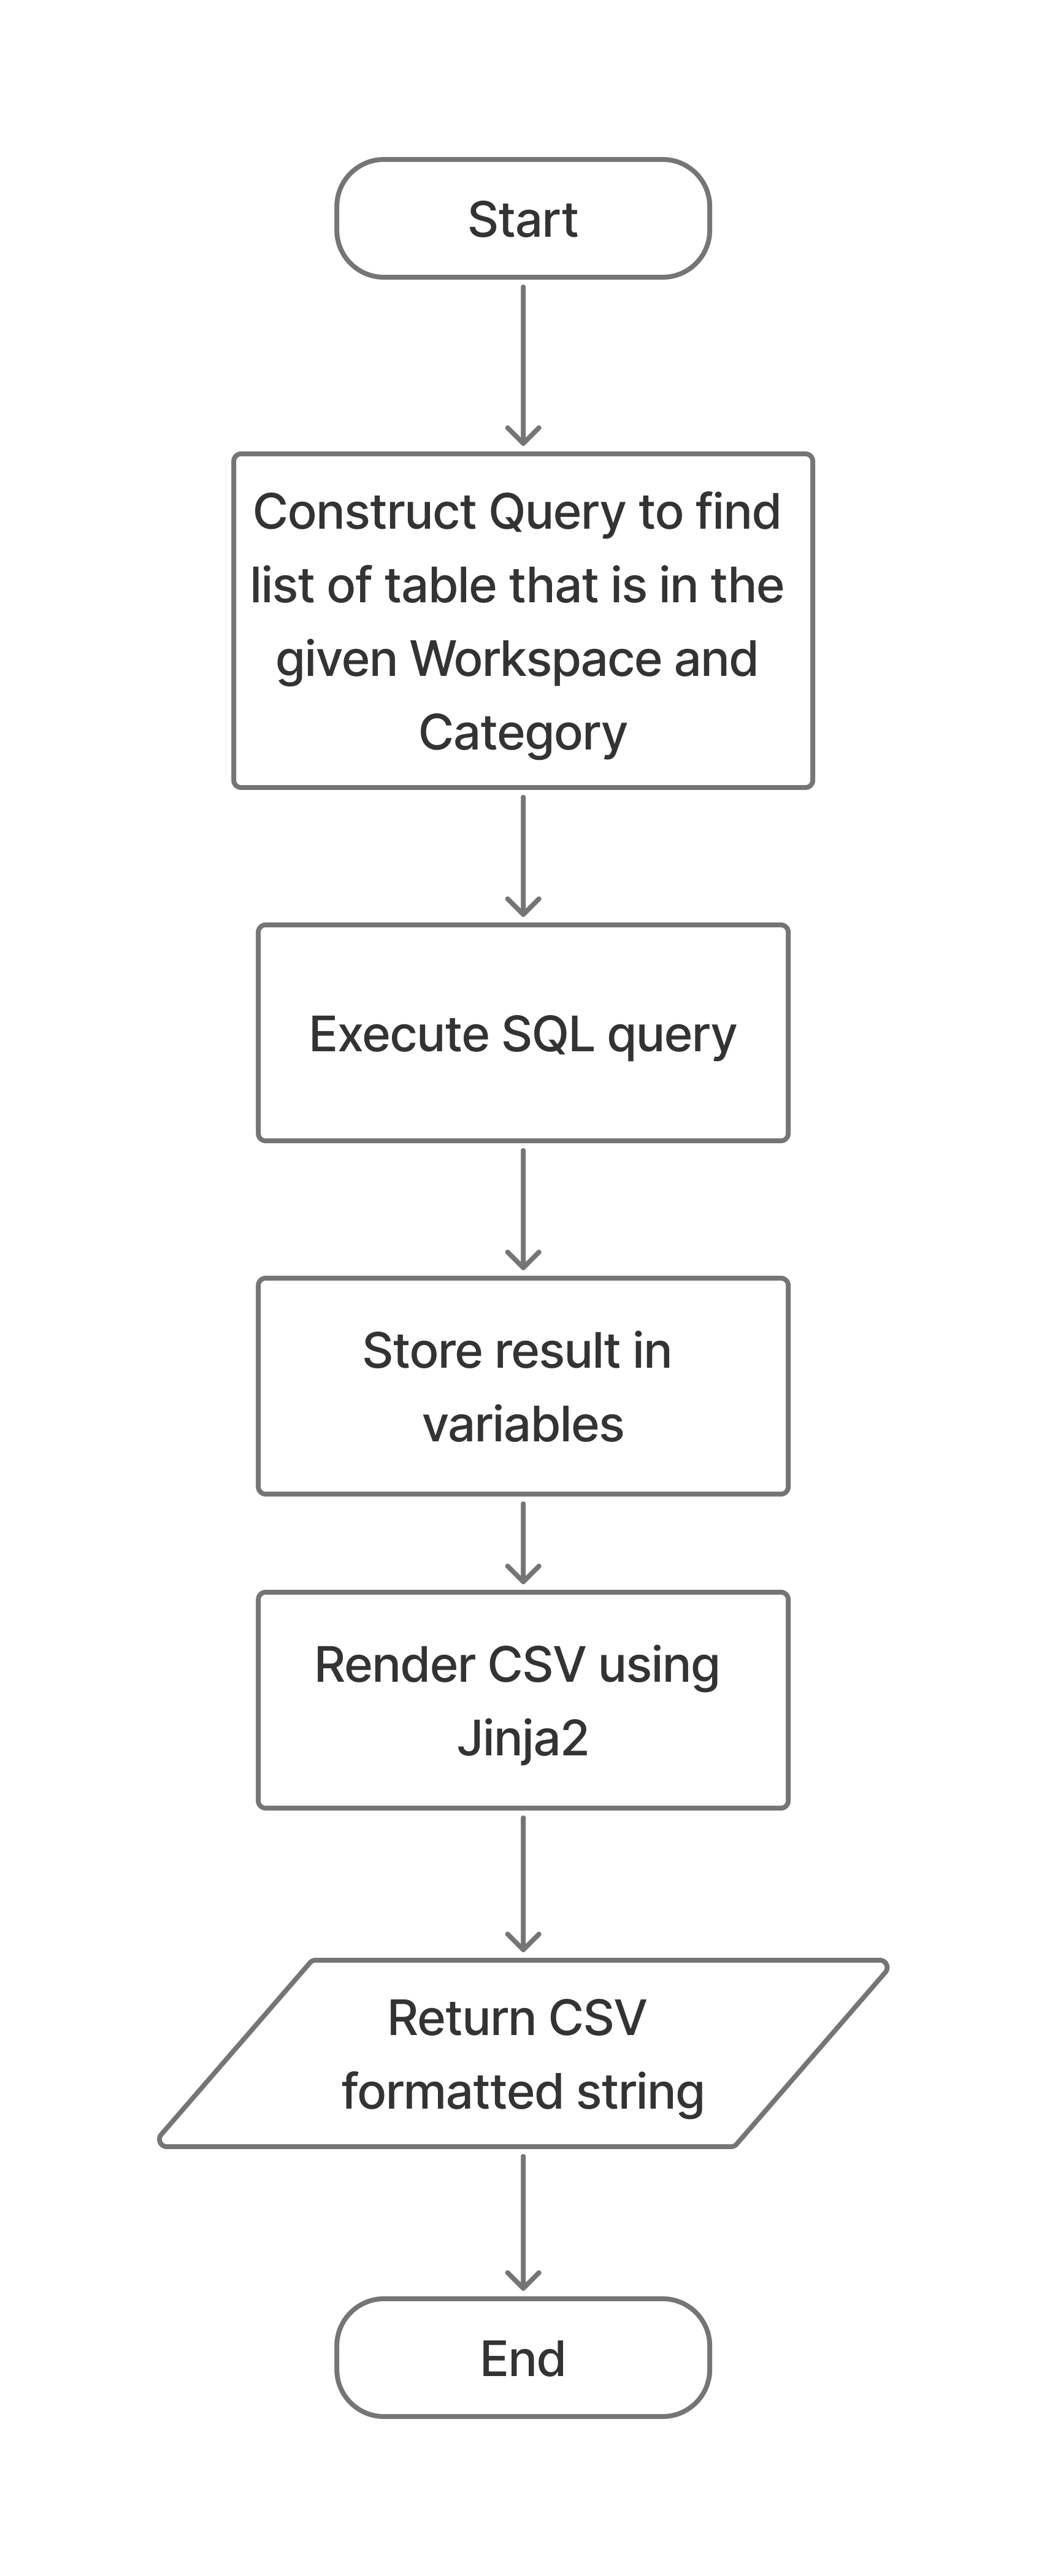
\includegraphics[width=5cm]{chapters/3/figures/table_in_workspace.jpg}
        \caption[Retrieve table in workspace tool’s flowchart]{Retrieve table in workspace tool’s flowchart}
        \label{fig:table_in_workspace}
    \end{figure}
    Figure~\ref{fig:table_in_workspace} This tool is used to retrieve tables that belong to a specific workspace. A workspace serves as a pre-filtering category, allowing you to narrow down the list of tables before searching for more detailed information about them. The tool returns a list of tables within the selected workspace, along with their descriptions, ordered by usage.

    Here is the breakdown of the flow:
    \begin{itemize}
        \item  SQL query is constructed to retrieve the list of tables that belong to the specified workspace and category. This step ensures that only relevant tables are selected based on the user's input or selection.
        \item  The constructed SQL query is executed 
        \item  The results returned from the SQL query are stored in variables for further processing.
        \item  The stored results are formatted into a CSV (Comma-Separated Values) string using the Jinja2 templating engine.
        \item  The final CSV-formatted string, which contains the list of tables and their details, is returned as the output of the tool.
    \end{itemize}

    \subsection{Retrieve chart summary}
    \label{sec:chart_summary}
    \begin{figure}[H]
        \centering
        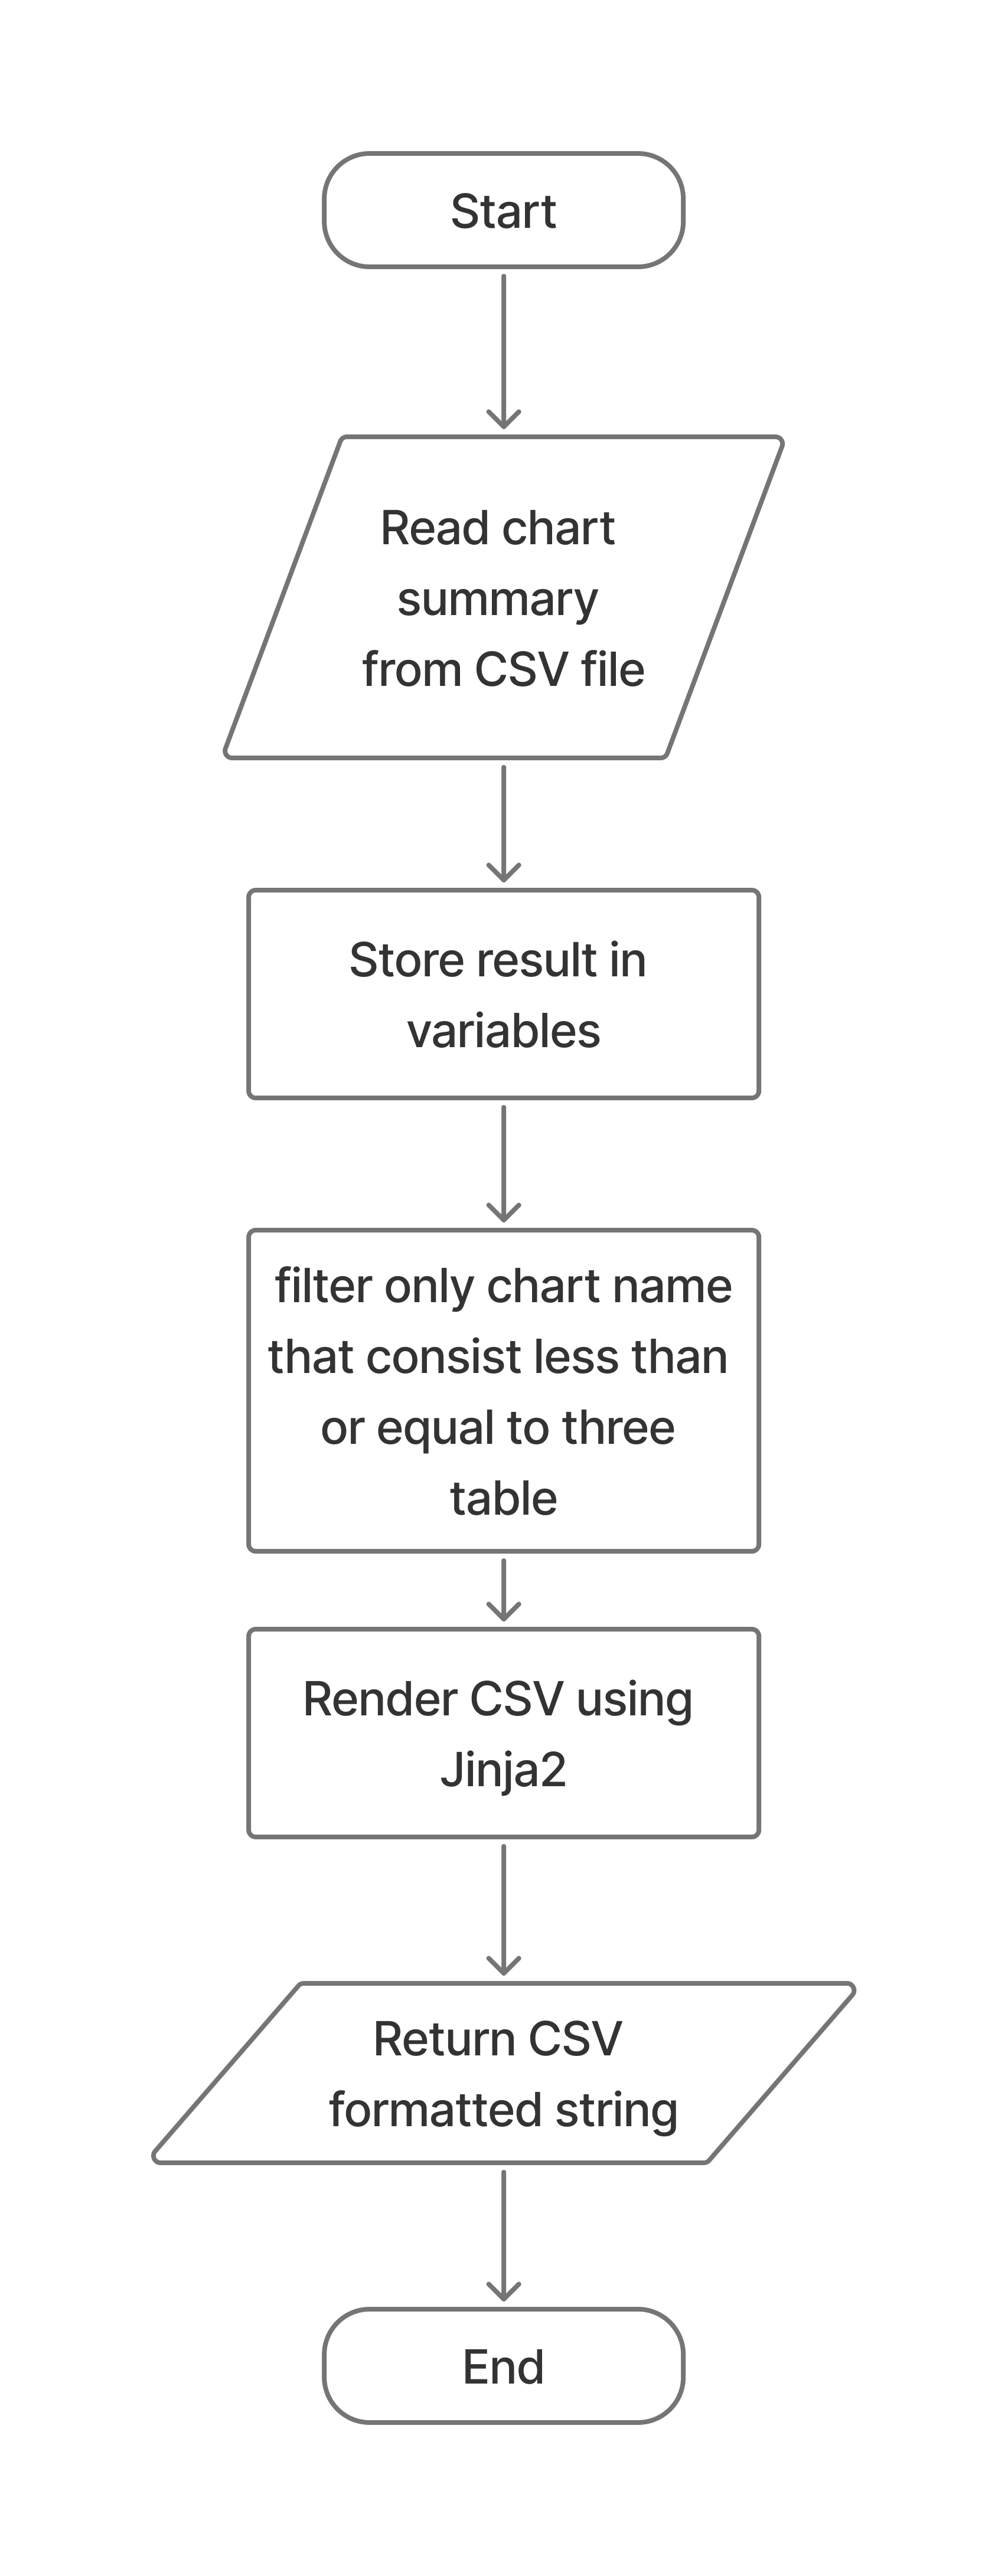
\includegraphics[width=5cm]{chapters/3/figures/chart_summary.jpg}
        \caption[Retrieve chart summary tool’s flowchart]{Retrieve chart summary tool’s flowchart}
        \label{fig:chart_summary}
    \end{figure}
    Figure~\ref{fig:chart_summary} This tool is used to retrieve additional business context based on the chart name summary provided by the user in Superset. It returns the business context, primary usage, and the related workspace and category.

    Here is the breakdown of the flow:
    \begin{itemize}
        \item  Import chart summary data from a CSV file.
        \item  Save the imported data into program variables for further use.
        \item  Select only those chart names that reference three or fewer tables.
        \item  Format the filtered data as a CSV string using the Jinja2 template engine..
        \item  Output the resulting CSV string.
    \end{itemize}

    \subsection{Pick Table}
    \label{sec:pick_table}
    \begin{figure}[H]
        \centering
        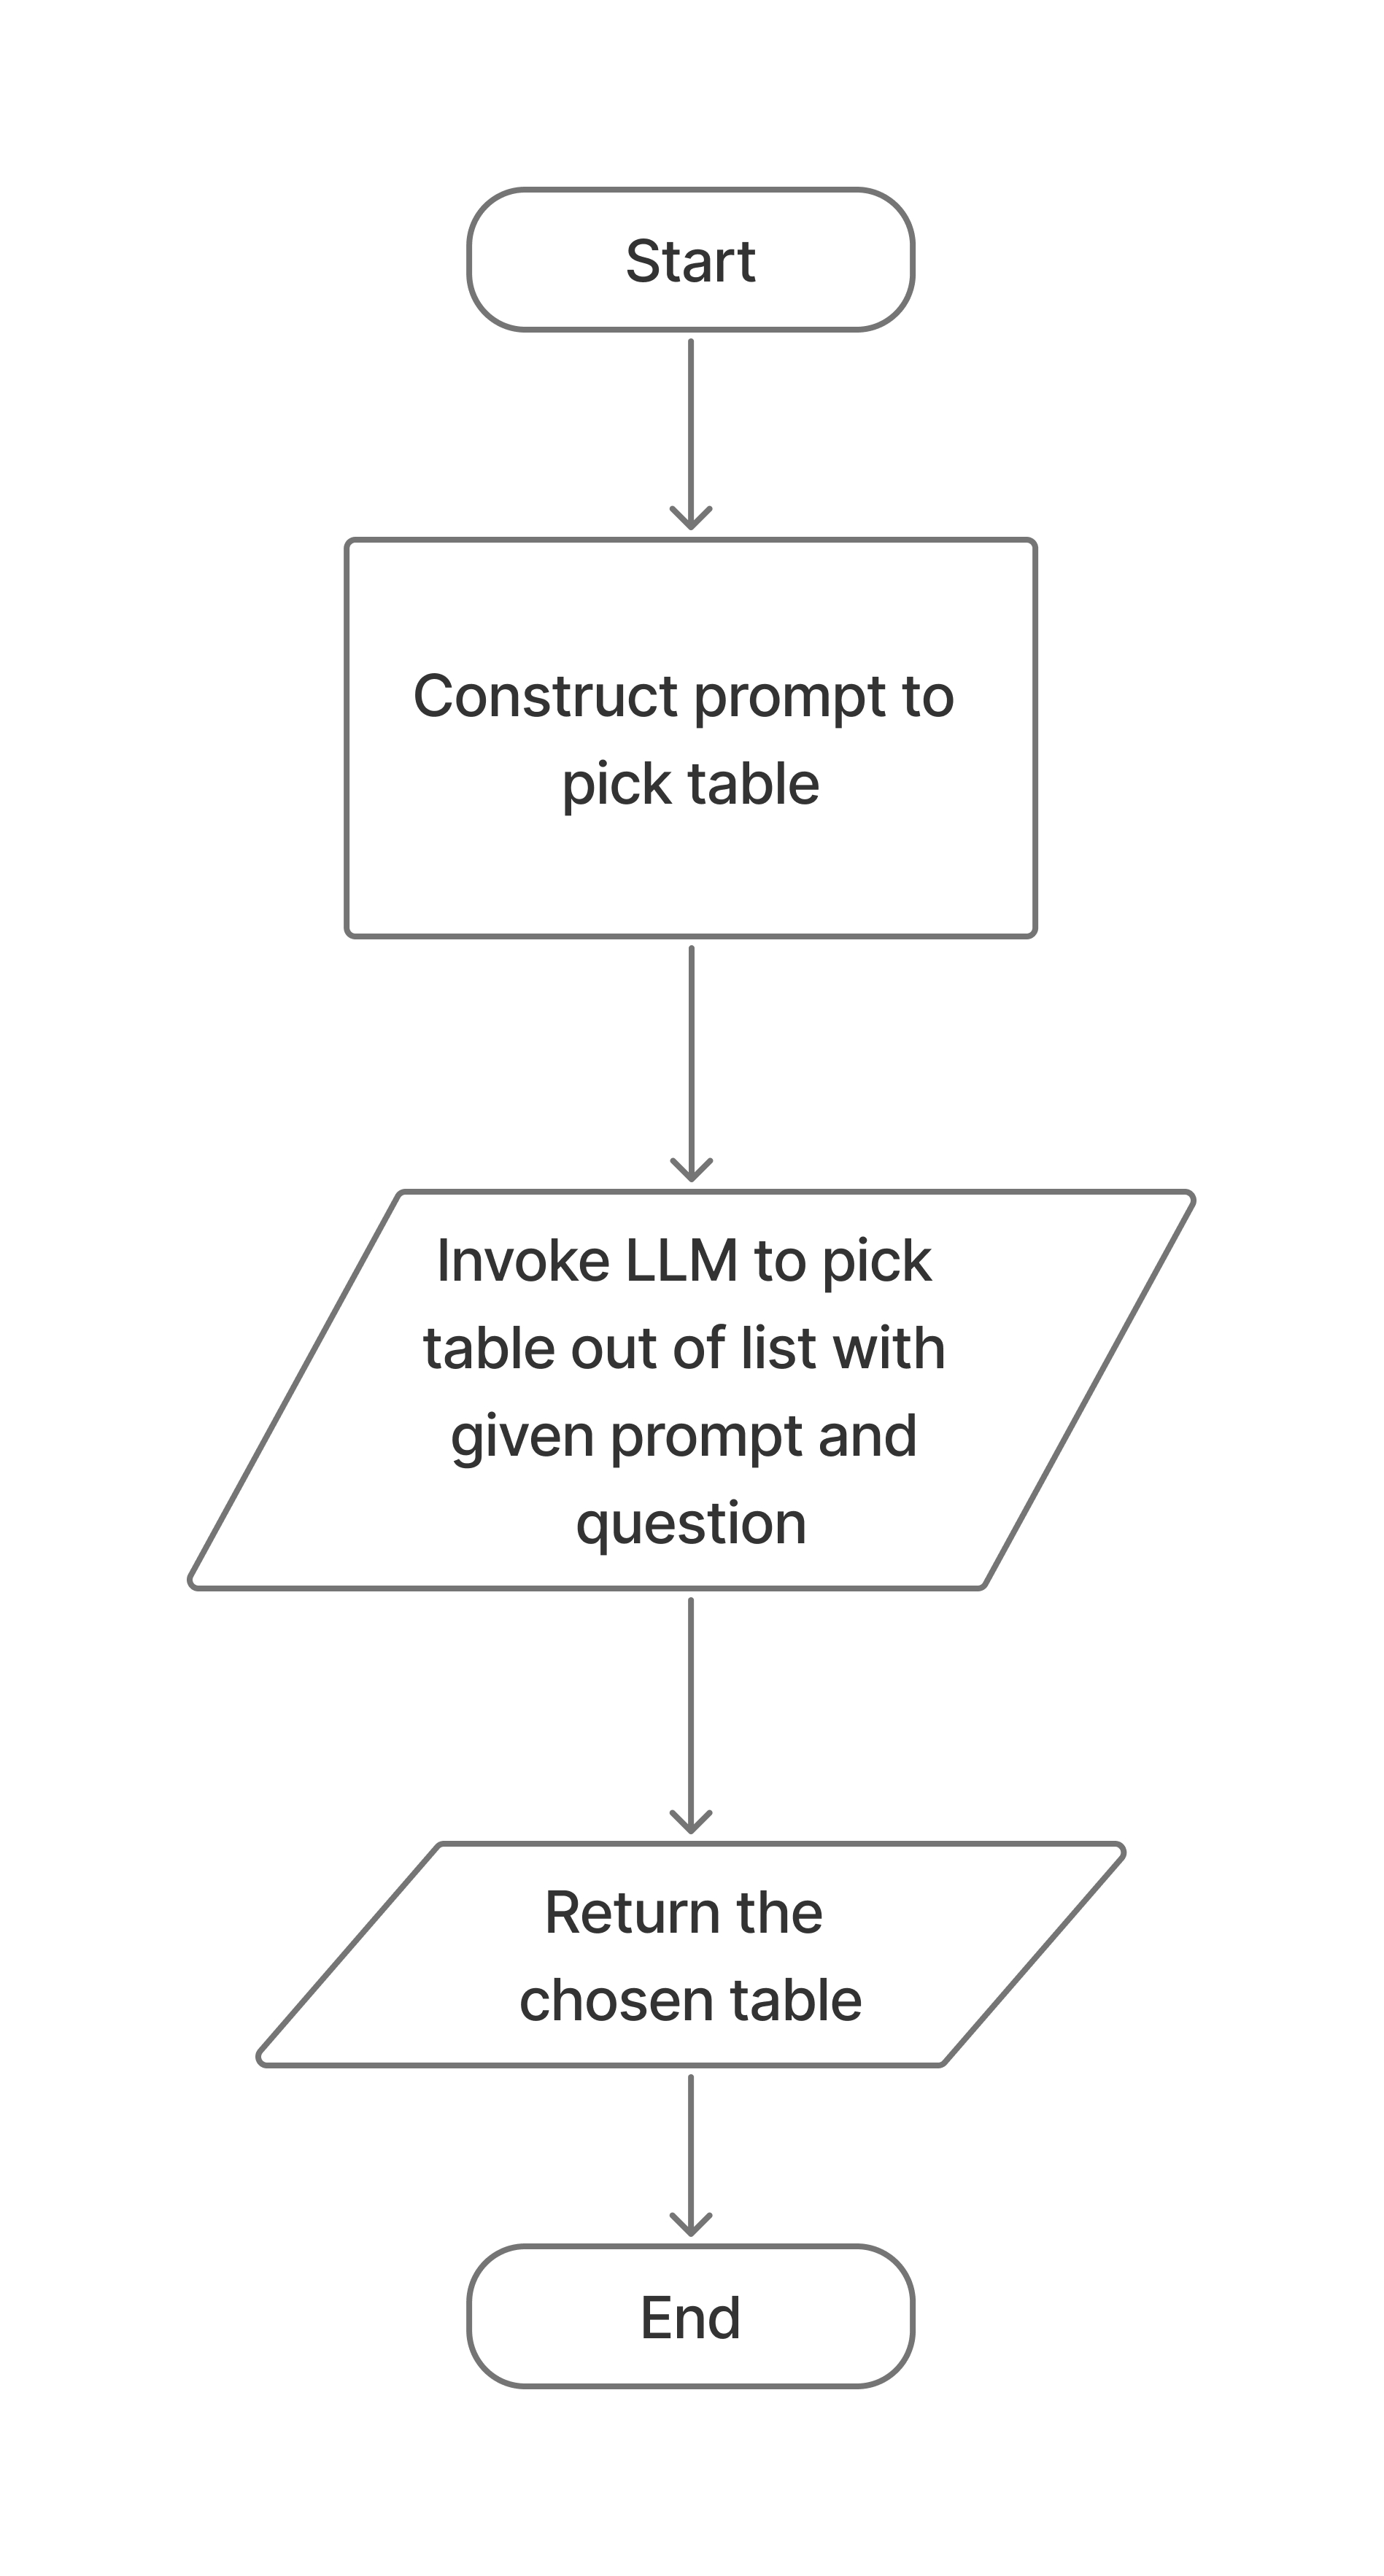
\includegraphics[width=5cm]{chapters/3/figures/pick_table.jpg}
        \caption[Pick Table tool’s flowchart]{Pick Table’s flowchart}
        \label{fig:pick_table}
    \end{figure}
    Figure~\ref{fig:pick_table} This tool is designed specifically to select tables by utilizing a separate LLM model, which can be more effective in choosing the appropriate table. This dedicated LLM focuses solely on table selection to answer the question, thereby reducing the workload of the main LLM agent.

    Here is the breakdown of the flow:
    \begin{itemize}
        \item  Prepare a prompt that will guide the table selection.
        \item  Invoke the LLM model with the prepared prompt.
        \item  Output the selected table as the result.
    \end{itemize}

\section{Phase 1}
    \subsection{Main Focus}
    In this phase, we focus on establishing the baseline for Query Assist, ensuring the system can detect and fix SQL errors while also handling syntax conversion between different query dialects. This involves implementing error-handling mechanisms, parsing query structures, and integrating rule-based or AI-driven approaches for syntax correction.

    To enhance query understanding and retrieval-augmented generation (RAG), we implement a PostgreSQL database to store metadata about tables and columns. This structured storage allows the system to retrieve relevant schema details, improving its ability to generate accurate query modifications.

    Additionally, we incorporate prompt tuning techniques to optimize interactions with the language model. By refining prompts, we enhance the model's ability to generate precise query transformations and improve overall system performance.

    By the end of this phase, the system should be capable of accurately identifying errors, converting queries to the appropriate format, and leveraging structured database knowledge to enhance SQL assistance.
    \subsection{Implementation}
    The implementation process of this phase began with constructing a baseline using LangChain and integrating the following tools:

    \begin{enumerate}
        \item \textbf{Retrieve Table Info} \\
        This function relies on Retrieval-Augmented Generation (RAG) to extract relevant table metadata. The implementation starts by constructing an SQL statement to fetch comprehensive table information. After retrieving the data, we apply cosine similarity to filter out only the columns that are most relevant to the search term.

        \item \textbf{Search Table} \\
        Similar to the previous tool, this function also utilizes RAG. The implementation begins with generating an SQL statement to fetch a list of tables. We then use cosine similarity to identify and rank tables that closely match the search term.

        \item \textbf{Validate Query} \\
        This tool connects to the database and executes the query using the \texttt{EXPLAIN} keyword. By analyzing the query execution plan, it determines whether the query contains errors, allowing for early detection and correction.
    \end{enumerate}
    \subsection{Slack Integration}
    The integration with Slack is achieved by developing a custom Slack bot designed to act as an intermediary between Slack and Query Assist. This bot facilitates seamless communication by handling the entire interaction process. When a user submits a query through Slack, the bot captures the input and sends it to Query Assist via an API. Once Query Assist processes the input and returns a response, the bot formats the output in a structured and user-friendly manner before posting it back to the appropriate Slack channel.

    In addition to managing the communication flow, the Slack bot is responsible for storing all relevant information in the messaging table. This includes user inputs, Query Assist responses, and any associated metadata, ensuring that all interactions are logged for future reference, analysis, and improvement of the system. By serving as a bridge between Slack and Query Assist, the bot ensures a streamlined and efficient user experience while maintaining a robust record of all query-related activities.
    \begin{figure}[H]
        \centering
        
\includegraphics[width=10cm]{chapters/3/figures/Slack-Logo.png}
        \caption[Slack]{Slack}
        \label{fig:slack-logo}
    \end{figure}
\section{Phase 2}
    \subsection{Main Focus}
    In this phase, the focus is on establishing the foundation for Query Assist to enable query generation from Natural Language inputs. This involves implementing methods for data selection and testing procedures to ensure the relevance and accuracy of generated queries.

    A combination of approaches is adopted, including fine-tuning a language model, leveraging workspace-based metadata, and incorporating conversation-driven query generation. These techniques are designed to refine the system's ability to interpret natural language and construct accurate SQL queries.

    To support schema understanding and selection for query construction, test cases are developed to validate the system's behavior across various scenarios. These test cases ensure robust functionality and reliable performance under different query inputs and metadata constraints.

    By the end of this phase, Query Assist is expected to effectively parse user intents, select relevant tables and columns, and generate precise SQL queries aligned with the provided data context.
    \subsection{Tools used}
    The number of tools used in this phase has increased, as additional tools are required to assist with table selection and related tasks. Some tools from Phase 1 are also shared in this phase. These tools were developed for testing purposes to determine the most effective approach for table selection.
    The following tools are utilized: 

    \begin{itemize}
        \item Pick Table tools in \ref{sec:pick_table}
        \item Retrieve Table in Workspace tools in \ref{sec:table_in_workspace}
        \item Retrieve Chart Summary tools in \ref{sec:chart_summary}
        \item Column Validation tools in \ref{sec:column_validation}
        \item Retrieve Table Information tools in \ref{sec:retrieve_table_info}
    \end{itemize}
    \subsection{Test Case Generation}
        \subsubsection{Table-Informed}
        In this method, test cases are generated by providing the table name to GPT, which then creates test cases based on the table's structure and purpose. Our objective is to generate 200 test cases from the top 100 most-used tables. The process involves the following steps:
        \begin{itemize}
            \item \textbf{Table Description Analysis:} Begin by providing GPT with a description of the table to gather details about its structure and columns.
            \item \textbf{Question Generation:} Prompt GPT to create specific, report-driven questions that focus on insights, trends, or summaries.
            \item \textbf{Specification of Tables and Columns:} For each question, clearly specify the table and the columns required to answer it.
            \item \textbf{Validation of Column Names:} Verify that the column names used in the generated questions actually exist in the table. This step ensures that the columns referenced are valid and present, as GPT may occasionally generate non-existent column names.
        \end{itemize}
        Additionally, real-world use cases derived from Opsbot tickets are provided as example questions to guide the generation process.

        To ensure the test cases reflect real-world usage, personas have been created for 11 departments within Agoda, based on internal knowledge. Each persona represents a specific group of users and their unique perspectives. Questions are generated from the perspective of these personas, ensuring they highlight deeper insights and align with actual use cases. This approach allows the test cases to better mimic real-world scenarios and address the key insights typically sought by users of the table.
        \subsubsection{Query-Informed}
        In this method, test cases are generated by filtering real-world user queries based on the most-used tables. The process aims to address the challenges of generating relevant test cases by maximally utilizing existing data. The process involves the following steps:
        \begin{itemize}
          \item \textbf{Table Scope Filtering:} Start by using OpenMetadata to check if a table has a description and ensure that at least 80\text{\%} of the table's columns are described. Only tables meeting both conditions are considered eligible.
          \item \textbf{Ranking by Usage:} Rank the filtered tables based on their usage frequency. Select the top 100 tables with the highest usage as the foundation for the test case generation.
          \item \textbf{Query Extraction:} Identify real user queries that involve these top 100 tables as input for generating detailed and realistic test cases.
          \item \textbf{Question Generation:} Utilize GPT to transform the filtered queries into specific, actionable test cases. The generated questions focus on insights, trends, or summaries derived from real user interactions.
          \item \textbf{Validation of Tables and Columns:} Verify that the tables and columns referenced in the generated questions exist and align with the actual structures of the involved tables. This step ensures accuracy and minimizes the risk of generating outputs that reference non-existent data.
        \end{itemize}
    \subsection{Chatting}
    A decision has been made to transition from a one-time interaction model to a conversational approach. This change enhances user engagement by transforming interactions into ongoing conversations. A user interface has been developed to test the model, enabling seamless conversational interactions. The model integrates its previous responses into new ones, allowing it to retain context and enabling users to continue the conversation without losing the flow.

    The primary objective of this transition is to allow users to provide feedback on GPT-generated answers. This feedback mechanism increases the likelihood of Query Assist delivering more accurate and precise responses over time, improving its overall effectiveness and reliability.
    \subsection{Workspace}
    Through research, the QueryGPT project \cite{QueryGPT} was identified as operating in a manner similar to this work. Their approach to selecting the appropriate table involves categorizing tables into workspaces, a method that has proven effective for their project. Drawing inspiration from this approach, a similar method was implemented by listing tables along with their descriptions and utilizing GPT to categorize them based on the provided descriptions.

    To further enhance table selection and organization, a two-tier filtering system has been developed. This system consists of the following filters:

    \begin{itemize}
        \item Workspace:

        The first filter, called 'Workspace' represents the primary grouping of tables and serves as the main product to be selected. Multiple workspaces can be chosen if the question or use case spans across them.
            \begin{itemize}
                \item Hotel \\
                Focused on tables containing information or data related to accommodations. This includes a wide range of lodging options such as hotels, hostels, vacation rentals, and other property types.
                \item Flight \\
                Dedicated to tables containing information or data related to flights. This includes data on flight bookings, schedules, pricing, financial transactions, promotions, and partnerships. The workspace supports all aspects of the flight booking service, ensuring comprehensive management of air travel-related data.

                \item {Activity} \\
                Designed for tables containing information or data related to activities and local experiences. This includes details about various activities, tours, and experiences that travelers can book to enhance their trips. The data may cover booking information, activity descriptions, pricing, availability, customer feedback, and promotional campaigns.

                \item {Technology and Development Insights} \\
                Provides a comprehensive view of Agoda's technology infrastructure, development processes, and IT operations. It brings together data from GitLab repositories, CI/CD pipelines, team structures, and system monitoring to support analysis of development efficiency, code quality, and operational health.

                \item {Workforce Analytics} \\
                Focused on employee performance, team structures, and workforce optimization.
            \end{itemize}

        \item Category

        The second filter, called "Category," involves selecting the appropriate category within each workspace. Categories provide a more granular classification of tables within a workspace. If a table does not belong to any category, no category is selected.
    \end{itemize}
    This two-tier system ensures a structured and efficient approach to mapping user questions to the appropriate tables, improving the accuracy and relevance of the results.

    \subsection{Fine-tuning}
    The fine-tuning method was introduced as a key development in this project following extensive research and analysis. This decision arose from observing limitations in existing tools, where search terms often failed to yield the desired tables and schema information. To address this issue, a fine-tuning model was developed to enhance the system’s ability to identify and suggest exact tables relevant to the query requirements.

    This approach builds upon the model's ability to learn from structured schema metadata, enabling it to provide more precise and contextually appropriate table selections. The introduction of fine-tuning lays the foundation for improved query generation, offering greater accuracy compared to relying solely on pre-existing search methods.

    By integrating the fine-tuning framework, the project ensures that Query Assist is capable of addressing specific user needs in table selection, thereby enhancing the reliability and effectiveness of SQL query construction.

% THIS IS AN EXAMPLE. ALL SECTIONS BELOW ARE OPTIONAL. PLEASE CONSULT YOU ADVISOR AND DESIGN YOUR OWN SECTION

% \emph{\textthai{หัวข้อต่าง ๆ ในแต่ละบทเป็นเพียงตัวอย่างเท่านั้น หัวข้อที่จะใส่ในแต่ละบทขึ้นอยู่กับโปรเจคของนักศึกษาและอาจารย์ที่ปรึกษา}}

% Explain the design (how you plan to implement your work) of your project. Adjust the section titles below to suit the types of your work. Detailed physical design like circuits and source codes should be placed in the appendix.

% \section{System Architecture}

%     \begin{table}[!h]
%         \centering
%         \caption{test table x1}\label{tbl:symbols}
%         \begin{tabular}{@{}p{0.07\textwidth}|p{0.7\textwidth}p{0.1\textwidth}}\hline
%         \multicolumn{2}{l}{\textbf{SYMBOL}}  & \textbf{UNIT} \\ \hline
%         $\alpha$ & Test variable\hfill & m$^2$ \\
%         $\lambda$ & Interarrival rate\hfill &  jobs/second\\
%         $\mu$ & Service rate\hfill & jobs/second \\ \hline
%         \end{tabular}
%         %\begin{tabular}{c|c} \hline
%         % $\alpha$ & $\beta$ \\ \hline
%         % $\delta$ & $\mu$ \\ \hline
%         %\end{tabular}
%     \end{table}

% \section{System Specifications and Requirements}

% \pagebreak
% \section{Hardware Module 1}
%     \emptyline 2
%     \subsection{Component 1}
%         \emptyline 2
%     \subsection{Logical Circuit Diagram}
%         \emptyline 2
% \pagebreak
% \section{Hardware Module 2}
%     \emptyline 2
%     \subsection{Component 1}
%         \emptyline 2
%     \subsection{Component 2}
%         \emptyline 2
% \pagebreak
% \section{Path Finding Algorithm}

% \pagebreak
% \section{Database Design}

% \pagebreak
% \section{GUI Design}

% \pagebreak
